% Options for packages loaded elsewhere
% Options for packages loaded elsewhere
\PassOptionsToPackage{unicode}{hyperref}
\PassOptionsToPackage{hyphens}{url}
\PassOptionsToPackage{dvipsnames,svgnames,x11names}{xcolor}
%
\documentclass[
]{article}
\usepackage{xcolor}
\usepackage{amsmath,amssymb}
\setcounter{secnumdepth}{5}
\usepackage{iftex}
\ifPDFTeX
  \usepackage[T1]{fontenc}
  \usepackage[utf8]{inputenc}
  \usepackage{textcomp} % provide euro and other symbols
\else % if luatex or xetex
  \usepackage{unicode-math} % this also loads fontspec
  \defaultfontfeatures{Scale=MatchLowercase}
  \defaultfontfeatures[\rmfamily]{Ligatures=TeX,Scale=1}
\fi
\usepackage{lmodern}
\ifPDFTeX\else
  % xetex/luatex font selection
\fi
% Use upquote if available, for straight quotes in verbatim environments
\IfFileExists{upquote.sty}{\usepackage{upquote}}{}
\IfFileExists{microtype.sty}{% use microtype if available
  \usepackage[]{microtype}
  \UseMicrotypeSet[protrusion]{basicmath} % disable protrusion for tt fonts
}{}
\makeatletter
\@ifundefined{KOMAClassName}{% if non-KOMA class
  \IfFileExists{parskip.sty}{%
    \usepackage{parskip}
  }{% else
    \setlength{\parindent}{0pt}
    \setlength{\parskip}{6pt plus 2pt minus 1pt}}
}{% if KOMA class
  \KOMAoptions{parskip=half}}
\makeatother
% Make \paragraph and \subparagraph free-standing
\makeatletter
\ifx\paragraph\undefined\else
  \let\oldparagraph\paragraph
  \renewcommand{\paragraph}{
    \@ifstar
      \xxxParagraphStar
      \xxxParagraphNoStar
  }
  \newcommand{\xxxParagraphStar}[1]{\oldparagraph*{#1}\mbox{}}
  \newcommand{\xxxParagraphNoStar}[1]{\oldparagraph{#1}\mbox{}}
\fi
\ifx\subparagraph\undefined\else
  \let\oldsubparagraph\subparagraph
  \renewcommand{\subparagraph}{
    \@ifstar
      \xxxSubParagraphStar
      \xxxSubParagraphNoStar
  }
  \newcommand{\xxxSubParagraphStar}[1]{\oldsubparagraph*{#1}\mbox{}}
  \newcommand{\xxxSubParagraphNoStar}[1]{\oldsubparagraph{#1}\mbox{}}
\fi
\makeatother


\usepackage{longtable,booktabs,array}
\usepackage{calc} % for calculating minipage widths
% Correct order of tables after \paragraph or \subparagraph
\usepackage{etoolbox}
\makeatletter
\patchcmd\longtable{\par}{\if@noskipsec\mbox{}\fi\par}{}{}
\makeatother
% Allow footnotes in longtable head/foot
\IfFileExists{footnotehyper.sty}{\usepackage{footnotehyper}}{\usepackage{footnote}}
\makesavenoteenv{longtable}
\usepackage{graphicx}
\makeatletter
\newsavebox\pandoc@box
\newcommand*\pandocbounded[1]{% scales image to fit in text height/width
  \sbox\pandoc@box{#1}%
  \Gscale@div\@tempa{\textheight}{\dimexpr\ht\pandoc@box+\dp\pandoc@box\relax}%
  \Gscale@div\@tempb{\linewidth}{\wd\pandoc@box}%
  \ifdim\@tempb\p@<\@tempa\p@\let\@tempa\@tempb\fi% select the smaller of both
  \ifdim\@tempa\p@<\p@\scalebox{\@tempa}{\usebox\pandoc@box}%
  \else\usebox{\pandoc@box}%
  \fi%
}
% Set default figure placement to htbp
\def\fps@figure{htbp}
\makeatother


% definitions for citeproc citations
\NewDocumentCommand\citeproctext{}{}
\NewDocumentCommand\citeproc{mm}{%
  \begingroup\def\citeproctext{#2}\cite{#1}\endgroup}
\makeatletter
 % allow citations to break across lines
 \let\@cite@ofmt\@firstofone
 % avoid brackets around text for \cite:
 \def\@biblabel#1{}
 \def\@cite#1#2{{#1\if@tempswa , #2\fi}}
\makeatother
\newlength{\cslhangindent}
\setlength{\cslhangindent}{1.5em}
\newlength{\csllabelwidth}
\setlength{\csllabelwidth}{3em}
\newenvironment{CSLReferences}[2] % #1 hanging-indent, #2 entry-spacing
 {\begin{list}{}{%
  \setlength{\itemindent}{0pt}
  \setlength{\leftmargin}{0pt}
  \setlength{\parsep}{0pt}
  % turn on hanging indent if param 1 is 1
  \ifodd #1
   \setlength{\leftmargin}{\cslhangindent}
   \setlength{\itemindent}{-1\cslhangindent}
  \fi
  % set entry spacing
  \setlength{\itemsep}{#2\baselineskip}}}
 {\end{list}}
\usepackage{calc}
\newcommand{\CSLBlock}[1]{\hfill\break\parbox[t]{\linewidth}{\strut\ignorespaces#1\strut}}
\newcommand{\CSLLeftMargin}[1]{\parbox[t]{\csllabelwidth}{\strut#1\strut}}
\newcommand{\CSLRightInline}[1]{\parbox[t]{\linewidth - \csllabelwidth}{\strut#1\strut}}
\newcommand{\CSLIndent}[1]{\hspace{\cslhangindent}#1}



\setlength{\emergencystretch}{3em} % prevent overfull lines

\providecommand{\tightlist}{%
  \setlength{\itemsep}{0pt}\setlength{\parskip}{0pt}}



 


\usepackage{booktabs}
\usepackage{longtable}
\usepackage{array}
\usepackage{multirow}
\usepackage{wrapfig}
\usepackage{float}
\usepackage{colortbl}
\usepackage{pdflscape}
\usepackage{tabu}
\usepackage{threeparttable}
\usepackage{threeparttablex}
\usepackage[normalem]{ulem}
\usepackage{makecell}
\usepackage{xcolor}
\usepackage{xcolor}
\usepackage{lscape}
\newcommand{\blandscape}{\begin{landscape}}
\newcommand{\elandscape}{\end{landscape}}
\usepackage{geometry}
\geometry{
  top=2.5cm,
  bottom=2.5cm,
  left=2.5cm,
  right=2.5cm
}
\makeatletter
\@ifpackageloaded{caption}{}{\usepackage{caption}}
\AtBeginDocument{%
\ifdefined\contentsname
  \renewcommand*\contentsname{Table of contents}
\else
  \newcommand\contentsname{Table of contents}
\fi
\ifdefined\listfigurename
  \renewcommand*\listfigurename{List of Figures}
\else
  \newcommand\listfigurename{List of Figures}
\fi
\ifdefined\listtablename
  \renewcommand*\listtablename{List of Tables}
\else
  \newcommand\listtablename{List of Tables}
\fi
\ifdefined\figurename
  \renewcommand*\figurename{Figure}
\else
  \newcommand\figurename{Figure}
\fi
\ifdefined\tablename
  \renewcommand*\tablename{Table}
\else
  \newcommand\tablename{Table}
\fi
}
\@ifpackageloaded{float}{}{\usepackage{float}}
\floatstyle{ruled}
\@ifundefined{c@chapter}{\newfloat{codelisting}{h}{lop}}{\newfloat{codelisting}{h}{lop}[chapter]}
\floatname{codelisting}{Listing}
\newcommand*\listoflistings{\listof{codelisting}{List of Listings}}
\makeatother
\makeatletter
\makeatother
\makeatletter
\@ifpackageloaded{caption}{}{\usepackage{caption}}
\@ifpackageloaded{subcaption}{}{\usepackage{subcaption}}
\makeatother
\usepackage{bookmark}
\IfFileExists{xurl.sty}{\usepackage{xurl}}{} % add URL line breaks if available
\urlstyle{same}
\hypersetup{
  pdftitle={Quantifying the accuracy of OpenStreetMap for longitudinal cycling-infrastructure change: A reproducible validation framework using Google Street View},
  pdfkeywords={OpenStreetMap (OSM), Volunteered geographic information
(VGI), Cycling infrastructure, Urban data science, Change
detection, Spatial validation, Reproducible workflows},
  colorlinks=true,
  linkcolor={blue},
  filecolor={Maroon},
  citecolor={Blue},
  urlcolor={Blue},
  pdfcreator={LaTeX via pandoc}}


\title{Quantifying the accuracy of OpenStreetMap for longitudinal
cycling-infrastructure change: A reproducible validation framework using
Google Street View}
\author{}
\date{}
\begin{document}
\maketitle
\begin{abstract}
Cities are rapidly expanding their cycling networks to promote
sustainable mobility, yet robust longitudinal data needed to evaluate
change are scarce. OpenStreetMap (OSM) provides a global, time-stamped
record of urban infrastructure, but its reliability for detecting change
over time remains uncertain. This study quantified the temporal accuracy
of OSM for identifying cycling-infrastructure additions and removals,
using Barcelona (2015--2023) as a case study within a reproducible
open-source workflow.

We reconstructed baseline and follow-up cycling networks from dated OSM
snapshots and applied geometric differencing to detect change. A
stratified sampling design, incorporating population density and urban
centrality, was used to validate detected changes against historical
Google Street View (GSV) imagery, allowing estimation of precision,
recall, and F1 scores. OSM-derived estimates indicate an 80.3\% increase
in cycling-infrastructure length, from 130.7 km to 235.7 km. For
additions, validation shows high recall (0.96) and strong precision
(0.82), indicating that OSM captures most real network expansions. For
removals, recall is high (1.00) but precision is notably low (0.20),
suggesting that many apparent losses reflect geometry edits or
re-tagging rather than physical infrastructure removal.

By explicitly quantifying detection accuracy, this study introduces a
transferable framework for calibrating OSM-based measures of
infrastructure change. The findings indicate that OSM snapshot
differencing can serve as a scalable screening approach for identifying
infrastructure additions, while apparent removals require cautious
interpretation and verification to avoid mapping artefacts being
mistaken for physical infrastructure loss. This calibration strengthens
longitudinal research by reducing exposure misclassification in public
health, transport safety, and urban equity.
\end{abstract}


\section{Introduction}\label{introduction}

In recent years, many cities worldwide have expanded their cycling
networks in pursuit of cleaner, healthier and more equitable mobility
(Szell et al. 2022; Buehler and Pucher 2021). Reliable data on how these
networks evolve are essential for evidence-based planning and robust
longitudinal research (Hirsch et al. 2016). Such data enable researchers
and policymakers to examine how infrastructure change relates to mode
choice, safety and equity (Houde, Apparicio, and Séguin 2018; Prince et
al. 2025).

Yet longitudinal infrastructure data are often incomplete or
inconsistent. Official inventories are rarely maintained systematically
across years, and field audits, although precise, are resource-intensive
and difficult to replicate at scale (Winters, Ferster, and Laberee 2025;
Dai et al. 2024). In the absence of consistent data, researchers and
policymakers must rely on fragmented sources, increasing the risk of
exposure misclassification and biased impact estimates (Batomen et al.
2026). As a result, comparable evidence on cycling-infrastructure change
remains limited, constraining both robust research and informed policy
development (Houde, Apparicio, and Séguin 2018).

The growing availability of Volunteered Geographic Information (VGI)
offers new opportunities to address these data gaps (Goodchild 2007).
Among such sources, OpenStreetMap (OSM) stands out for providing open,
editable, and time-stamped spatial data on a wide range of urban
features, making it a valuable resource for reconstructing historical
infrastructure networks and studying urban infrastructure change over
time (Minghini and Frassinelli 2019; Zhang and Pfoser 2019).

Early comparisons with authoritative datasets suggest that OSM can
achieve good positional accuracy and substantial agreement in mapped
features (Haklay 2010; Girres and Touya 2010). However, its use for
longitudinal change analysis remains more uncertain. OSM data quality
varies across space and time, and edits may reflect not only real-world
changes but also evolving mapping practices, including delayed or
retrospective updates (Barron, Neis, and Zipf 2014; Senaratne et al.
2017; Minghini and Frassinelli 2019). In addition, tagging practices and
compliance can vary across local contexts, introducing further
heterogeneity in how features are represented (Almendros-Jiménez and
Becerra-Terón 2018). This uncertainty in timing can influence analytical
results when historical OSM snapshots are used as proxies for real-world
change (Schmidl, Navratil, and Giannopoulos 2021; Juhász 2021).

Cycling infrastructure poses additional challenges because some
facilities, particularly on-street cycle lanes, are represented as
attributes of road segments rather than as independent geometries. This
makes them less visually distinct, harder to map consistently, and more
prone to omission or incorrect tagging (Hochmair, Zielstra, and Neis
2015; Ferster et al. 2023). Despite these challenges, empirical
comparisons with reference datasets suggest that OSM can provide useful
cycling-infrastructure inventories in many contexts, although agreement
varies across cities and infrastructure types and depends on consistent
tagging practices (Ferster et al. 2020). Evidence also suggests that OSM
bicycle-infrastructure data quality varies spatially, particularly
outside dense urban cores (Vierø, Vybornova, and Szell 2025).

Importantly, recent work has shown the value of OSM histories for
measuring cycling-network growth at scale, providing a scalable
alternative when consistent historical official datasets are unavailable
(Bres et al. 2023; Winters, Ferster, and Laberee 2025). At the same
time, these studies highlight that observed changes can reflect both
real-world infrastructure change and improvements in mapping and
tagging.

For this reason, OSM-derived changes require independent validation. To
assess whether changes detected from historical OSM snapshots reflect
real on-street changes, an external source of evidence is needed.
Street-level imagery, including Google Street View (GSV), has
increasingly been used to audit and validate built-environment features
remotely (Rundle et al. 2011; Askari et al. 2025; Hanibuchi, Nakaya, and
Inoue 2019). However, to our knowledge, no study has yet provided a
fully reproducible end-to-end workflow that combines OSM snapshot
differencing, probability-based stratified sampling, and GSV-based
verification to quantify precision and recall of cycling-infrastructure
change.

This study addresses this gap by quantifying the temporal accuracy of
OSM-derived cycling-infrastructure change. Using Barcelona over the
2015--2023 period as a case study, we implement a reproducible
open-source workflow that combines longitudinal snapshot differencing
with probability-based stratified validation against historical GSV
imagery. The selected time window aligns with a broader research project
examining infrastructure change across policy-relevant governance
periods, although the present paper focuses exclusively on
methodological validation. Detection performance is evaluated using
precision, recall, and F1 scores. By integrating change detection and
external validation within a transparent computational pipeline, the
study provides a transferable framework for calibrating OSM-based
measures of infrastructure change.

\section{Data and methods}\label{data-and-methods}

\subsection{Study setting}\label{study-setting}

Barcelona is a large, dense Mediterranean city in northeastern Spain
(around 1.7 million inhabitants within the municipal boundary) with an
extensive and evolving cycling network. Between 2015 and 2023, the city
experienced substantial cycling-infrastructure expansion, generating
measurable network change over time. These dynamics make Barcelona a
suitable case for evaluating OSM-based network reconstruction, change
detection, and validation procedures.

\subsection{Data sources}\label{data-sources}

Three data sources were used:

\begin{itemize}
\item
  \textbf{OpenStreetMap (OSM).} Dated OSM extracts for Barcelona were
  retrieved for 1 January 2016 and 1 January 2024 using the
  \texttt{osmextract} R package. These annual Geofabrik snapshots were
  used as proxies for baseline and follow-up network conditions.
\item
  \textbf{Google Street View (GSV).} Historical Street View panoramas
  were used to manually validate a sample of OSM-detected
  cycling-infrastructure additions and removals. Imagery corresponding
  as closely as possible to the baseline and follow-up reference periods
  was used for validation.
\item
  \textbf{Census and boundary data.} Census-tract boundaries (2015) and
  resident population counts (2022) were obtained from official
  statistical sources and used to design a stratified validation sample
  based on population density and centrality.
\end{itemize}

\subsection{Methods}\label{methods}

The analysis followed a five-step reproducible workflow
(Figure~\ref{fig-workflow}) with two main components: (i) temporal
differencing of dated OSM extracts to detect additions and removals of
cycling infrastructure, and (ii) stratified GSV validation to check a
sample of these detected changes.

\begin{figure}

\centering{

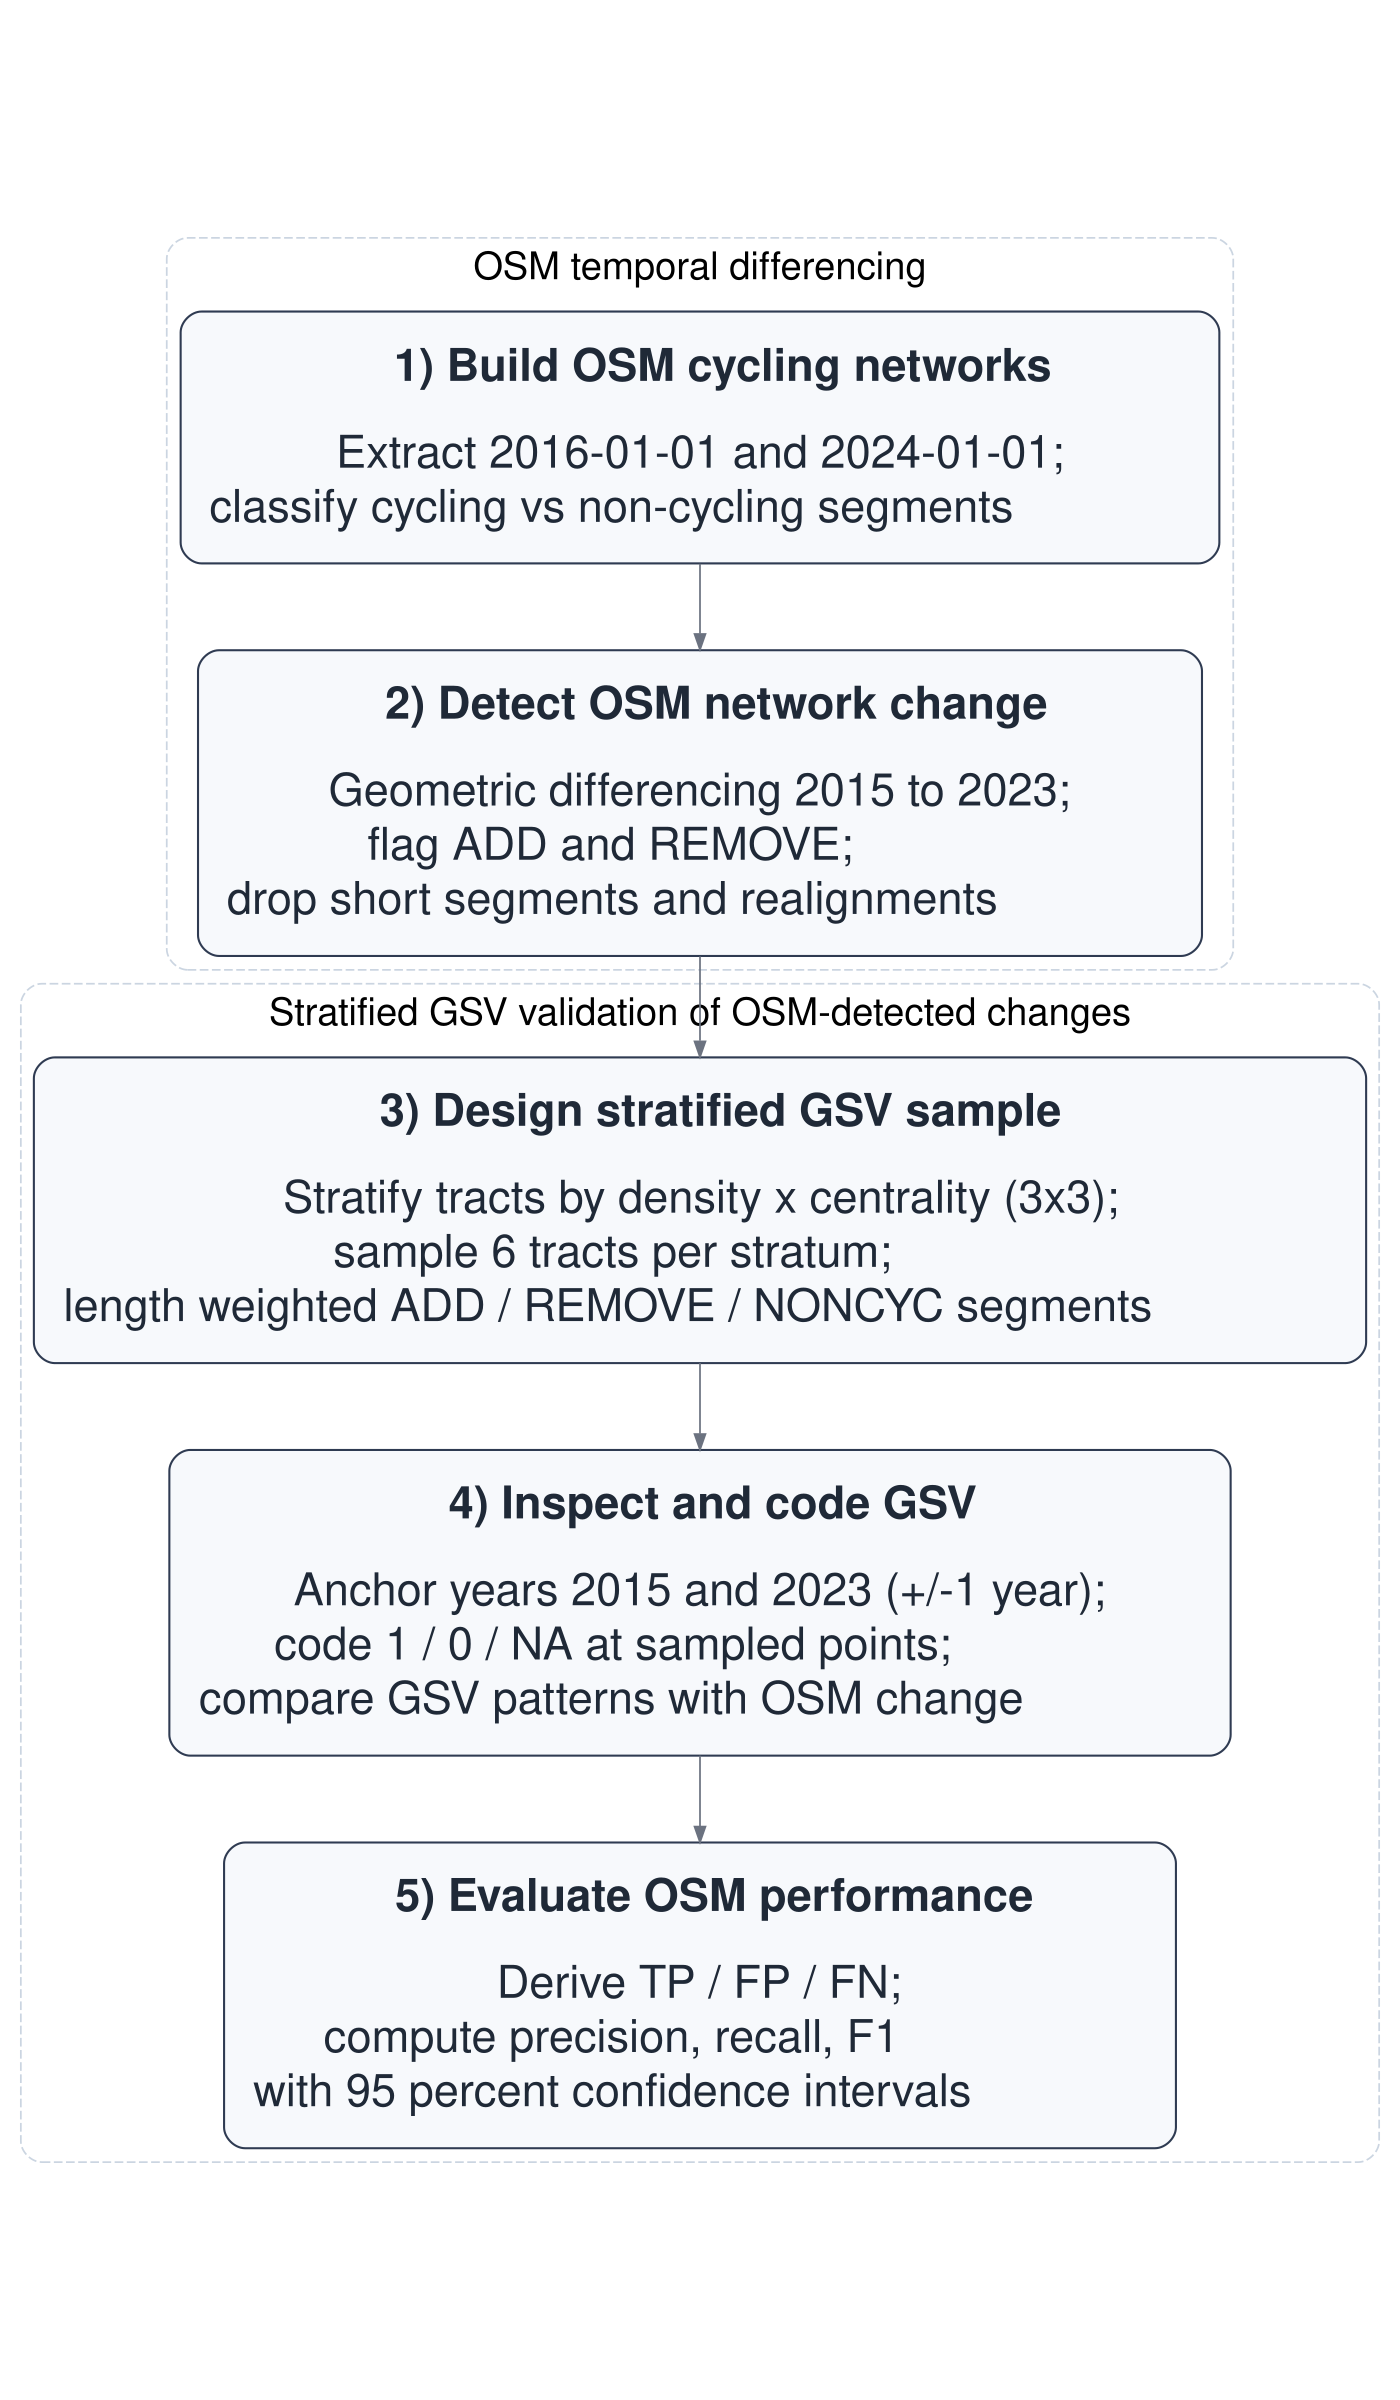
\includegraphics[width=0.5\linewidth,height=\textheight,keepaspectratio]{../figs/flowchart.png}

}

\caption{\label{fig-workflow}Main workflow steps.}

\end{figure}%

\subsubsection{OSM temporal
differencing}\label{osm-temporal-differencing}

\textbf{Step 1. Build OSM cycling networks}

We constructed baseline and follow-up cycling-infrastructure networks
from the dated OSM extracts described above, representing proxy
conditions for 2015 and 2023. From each extract, we derived a core
cycling-infrastructure network intended to represent bicycle-specific,
physically visible infrastructure encoded by the segment geometry. A
segment was classified as cycling infrastructure if either (i) it was
mapped as a dedicated cycleway (\texttt{highway\ =\ cycleway}), or (ii)
it was a street segment carrying explicit cycleway tags indicating a
lane or track. In the second case, we searched \texttt{cycleway}-related
keys (e.g., \texttt{cycleway}, \texttt{cycleway:left},
\texttt{cycleway:right}, \texttt{cycleway:both}, and other
\texttt{cycleway:*} variants) and retained segments where any value
matched \{\texttt{lane}, \texttt{track}, \texttt{opposite\_lane},
\texttt{opposite\_track}\} (OpenStreetMap contributors n.d.). Values
were matched case-insensitively and, where multiple values were present,
a segment was retained if any value matched the set above.

To reduce duplication from parallel OSM representations of the same
facility (e.g., a dedicated cycle track mapped as a separate geometry
while a cycle lane is also tagged on the adjacent carriageway), we
applied a no-double-counting (NDC) rule. Specifically, on-road
cycle-lane segments were excluded when they overlapped with nearby
dedicated cycling infrastructure, defined as cases where at least 20 m
of the lane segment and at least 50\% of its length fell within a 15 m
buffer around dedicated cycling geometries. The 15 m proximity threshold
reflects typical spatial offsets between carriageway-centreline
representations and adjacent segregated cycle tracks in dense urban
settings, while remaining conservative enough to avoid conflating
distinct facilities on opposite sides of wide corridors. The additional
requirements of a minimum 20 m overlap and at least 50\% segment
inclusion ensure that exclusions reflect substantive parallel
representation rather than incidental geometric proximity.

\textbf{Step 2. Detect OSM network change}

Cycling-infrastructure change between the baseline and follow-up
networks was detected using geometric differencing in a projected CRS.
First, each network was dissolved and buffered by 10 m to accommodate
minor geometric misalignments and small positional edits. This tolerance
absorbs small positional shifts introduced by re-digitisation or
geometry refinement, while remaining conservative relative to typical
urban carriageway widths. Additions were defined as segments present in
the 2023 proxy network but absent from the buffered 2015 proxy network;
removals were defined analogously as segments present in the 2015 proxy
network but absent from the buffered 2023 proxy network. Resulting
fragments shorter than 10 m were discarded.

To avoid counting positional edits in OSM as real infrastructure change,
we flagged likely realignments as cases where an added segment lay
within 15 m of a corresponding removed segment, reflecting small shifts
in mapped geometry rather than substantive infrastructure modification.
These cases were excluded from the validation evaluation pool. The 15 m
proximity threshold serves a distinct purpose from the differencing
buffer: it is intended to capture cases where added and removed
fragments likely represent the same infrastructure feature that has been
re-drawn, split, or slightly shifted in OSM rather than physically
removed and rebuilt.

To define control locations and support the identification of false
negatives, we constructed a non-cycling comparison pool (NONCYC)
consisting of general street segments that did not meet the
cycling-infrastructure tagging criteria. NONCYC candidates were
restricted to standard road classes (\texttt{highway} \(\in\)
\{\texttt{primary}, \texttt{secondary}, \texttt{tertiary},
\texttt{unclassified}, \texttt{residential} and corresponding link
classes, \texttt{living\_street}, \texttt{pedestrian}\}). To avoid
sampling road segments that overlap or lie immediately adjacent to
cycling infrastructure, we removed any NONCYC candidate geometries
located within 10 m of cycling infrastructure in either reference year
(2015 proxy or 2023 proxy). Resulting fragments shorter than 10 m were
discarded.

\subsubsection{Stratified GSV
validation}\label{stratified-gsv-validation}

\textbf{Step 3. Design stratified GSV sample}

To evaluate the accuracy of OSM-detected cycling-infrastructure changes,
we designed a stratified GSV validation across Barcelona's 1,063 census
tracts (2015; Figure~\ref{fig-strata-validation} a). Population density
was calculated as the 2022 resident population per square kilometre for
each tract, using official census counts and tract area. Centrality was
operationalised as a simple, reproducible proxy for inner vs outer
areas, measured via Euclidean distance to Plaça Catalunya. Each variable
was divided into terciles, and their combination produced nine
density--centrality strata (D1\_C1 to D3\_C3). From each stratum, six
tracts were randomly selected (total \(n = 54\)).

Within each sampled tract, we attempted to sample up to two OSM-detected
additions, two removals, and one NONCYC control segment. Segments were
sampled with probability proportional to their length, so longer
segments were more likely to be selected than shorter fragments.
Candidate segments were split at census-tract boundaries before sampling
so that segment length (and therefore sampling probability) was
calculated only within each tract.

Each sampled segment was converted to a single validation point located
at its mid-length position (Figure~\ref{fig-strata-validation} b).
Points were linked to the nearest available GSV panorama and exported to
a structured coding workbook (see Supplement
\hyperref[s1-workbook]{S1}). The same points were also provided in an
interactive map with direct Street View links (Supplement
\hyperref[s2-interactive-maps]{S2}).

\begin{figure}

\begin{minipage}{0.50\linewidth}

\centering{

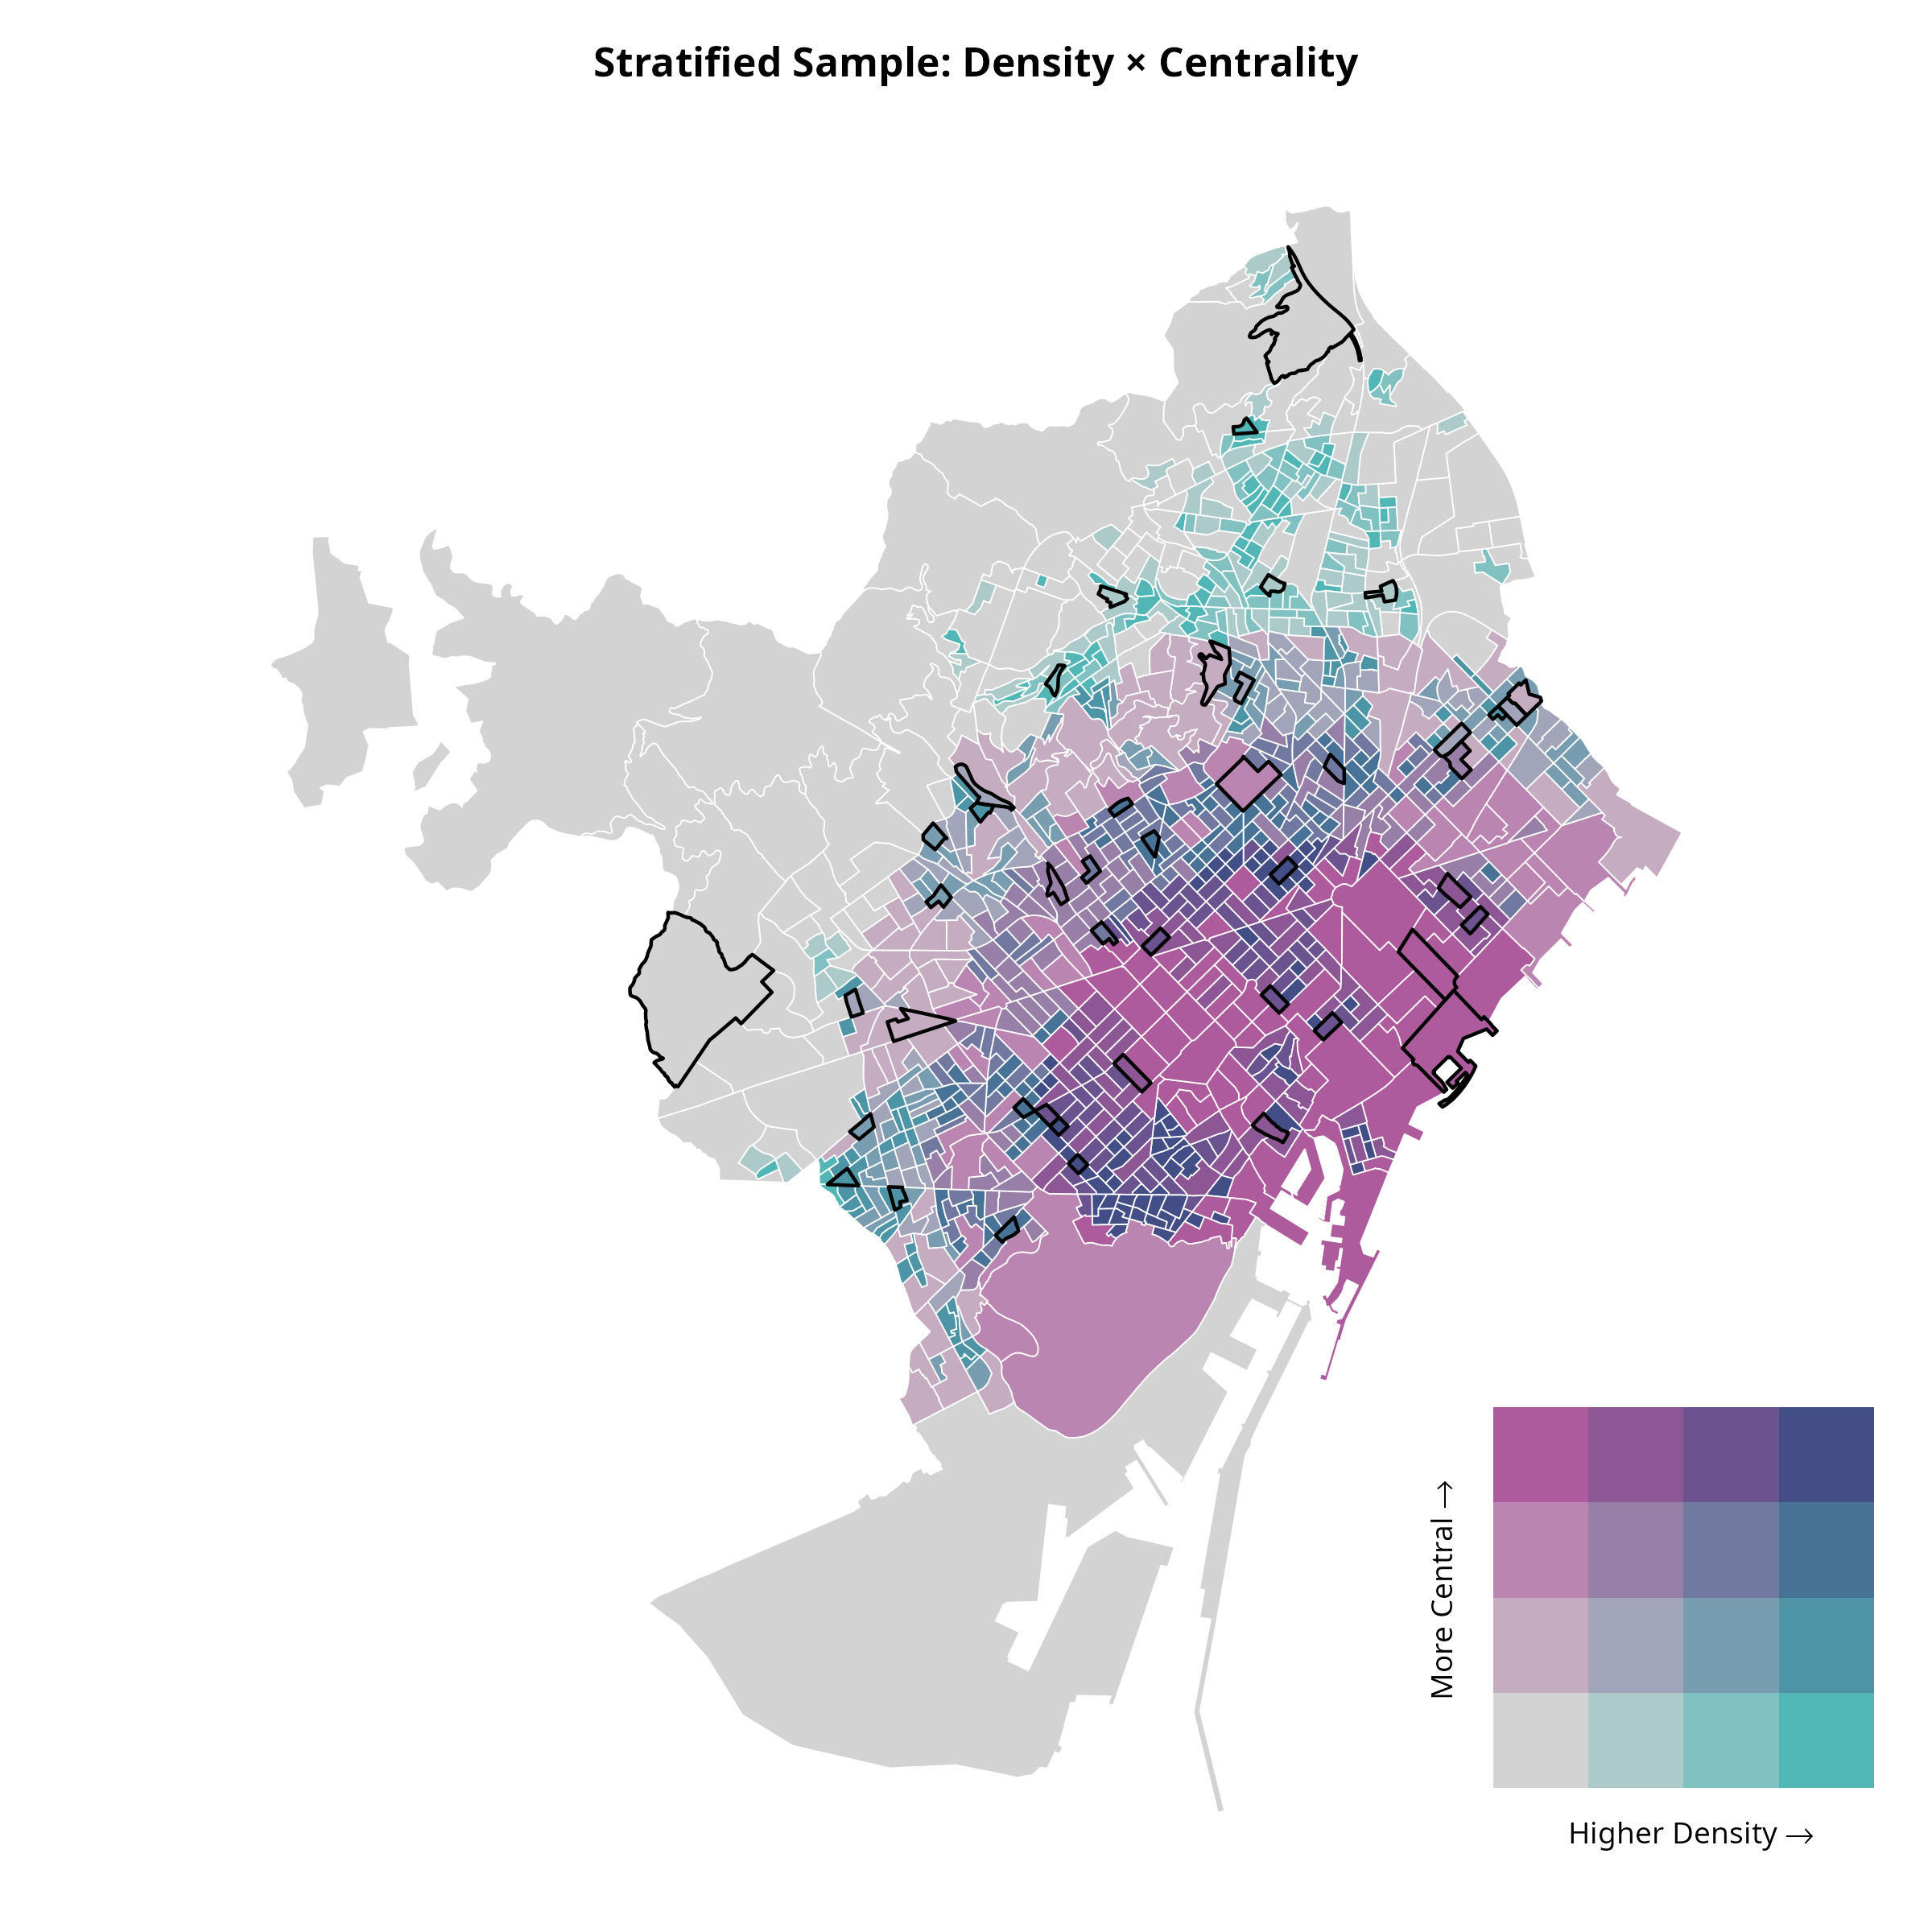
\includegraphics[width=1\linewidth,height=\textheight,keepaspectratio]{../figs/stratified_sample_bivariate_map.png}

}

\subcaption{\label{fig-strata-validation-1}}

\end{minipage}%
%
\begin{minipage}{0.50\linewidth}

\centering{

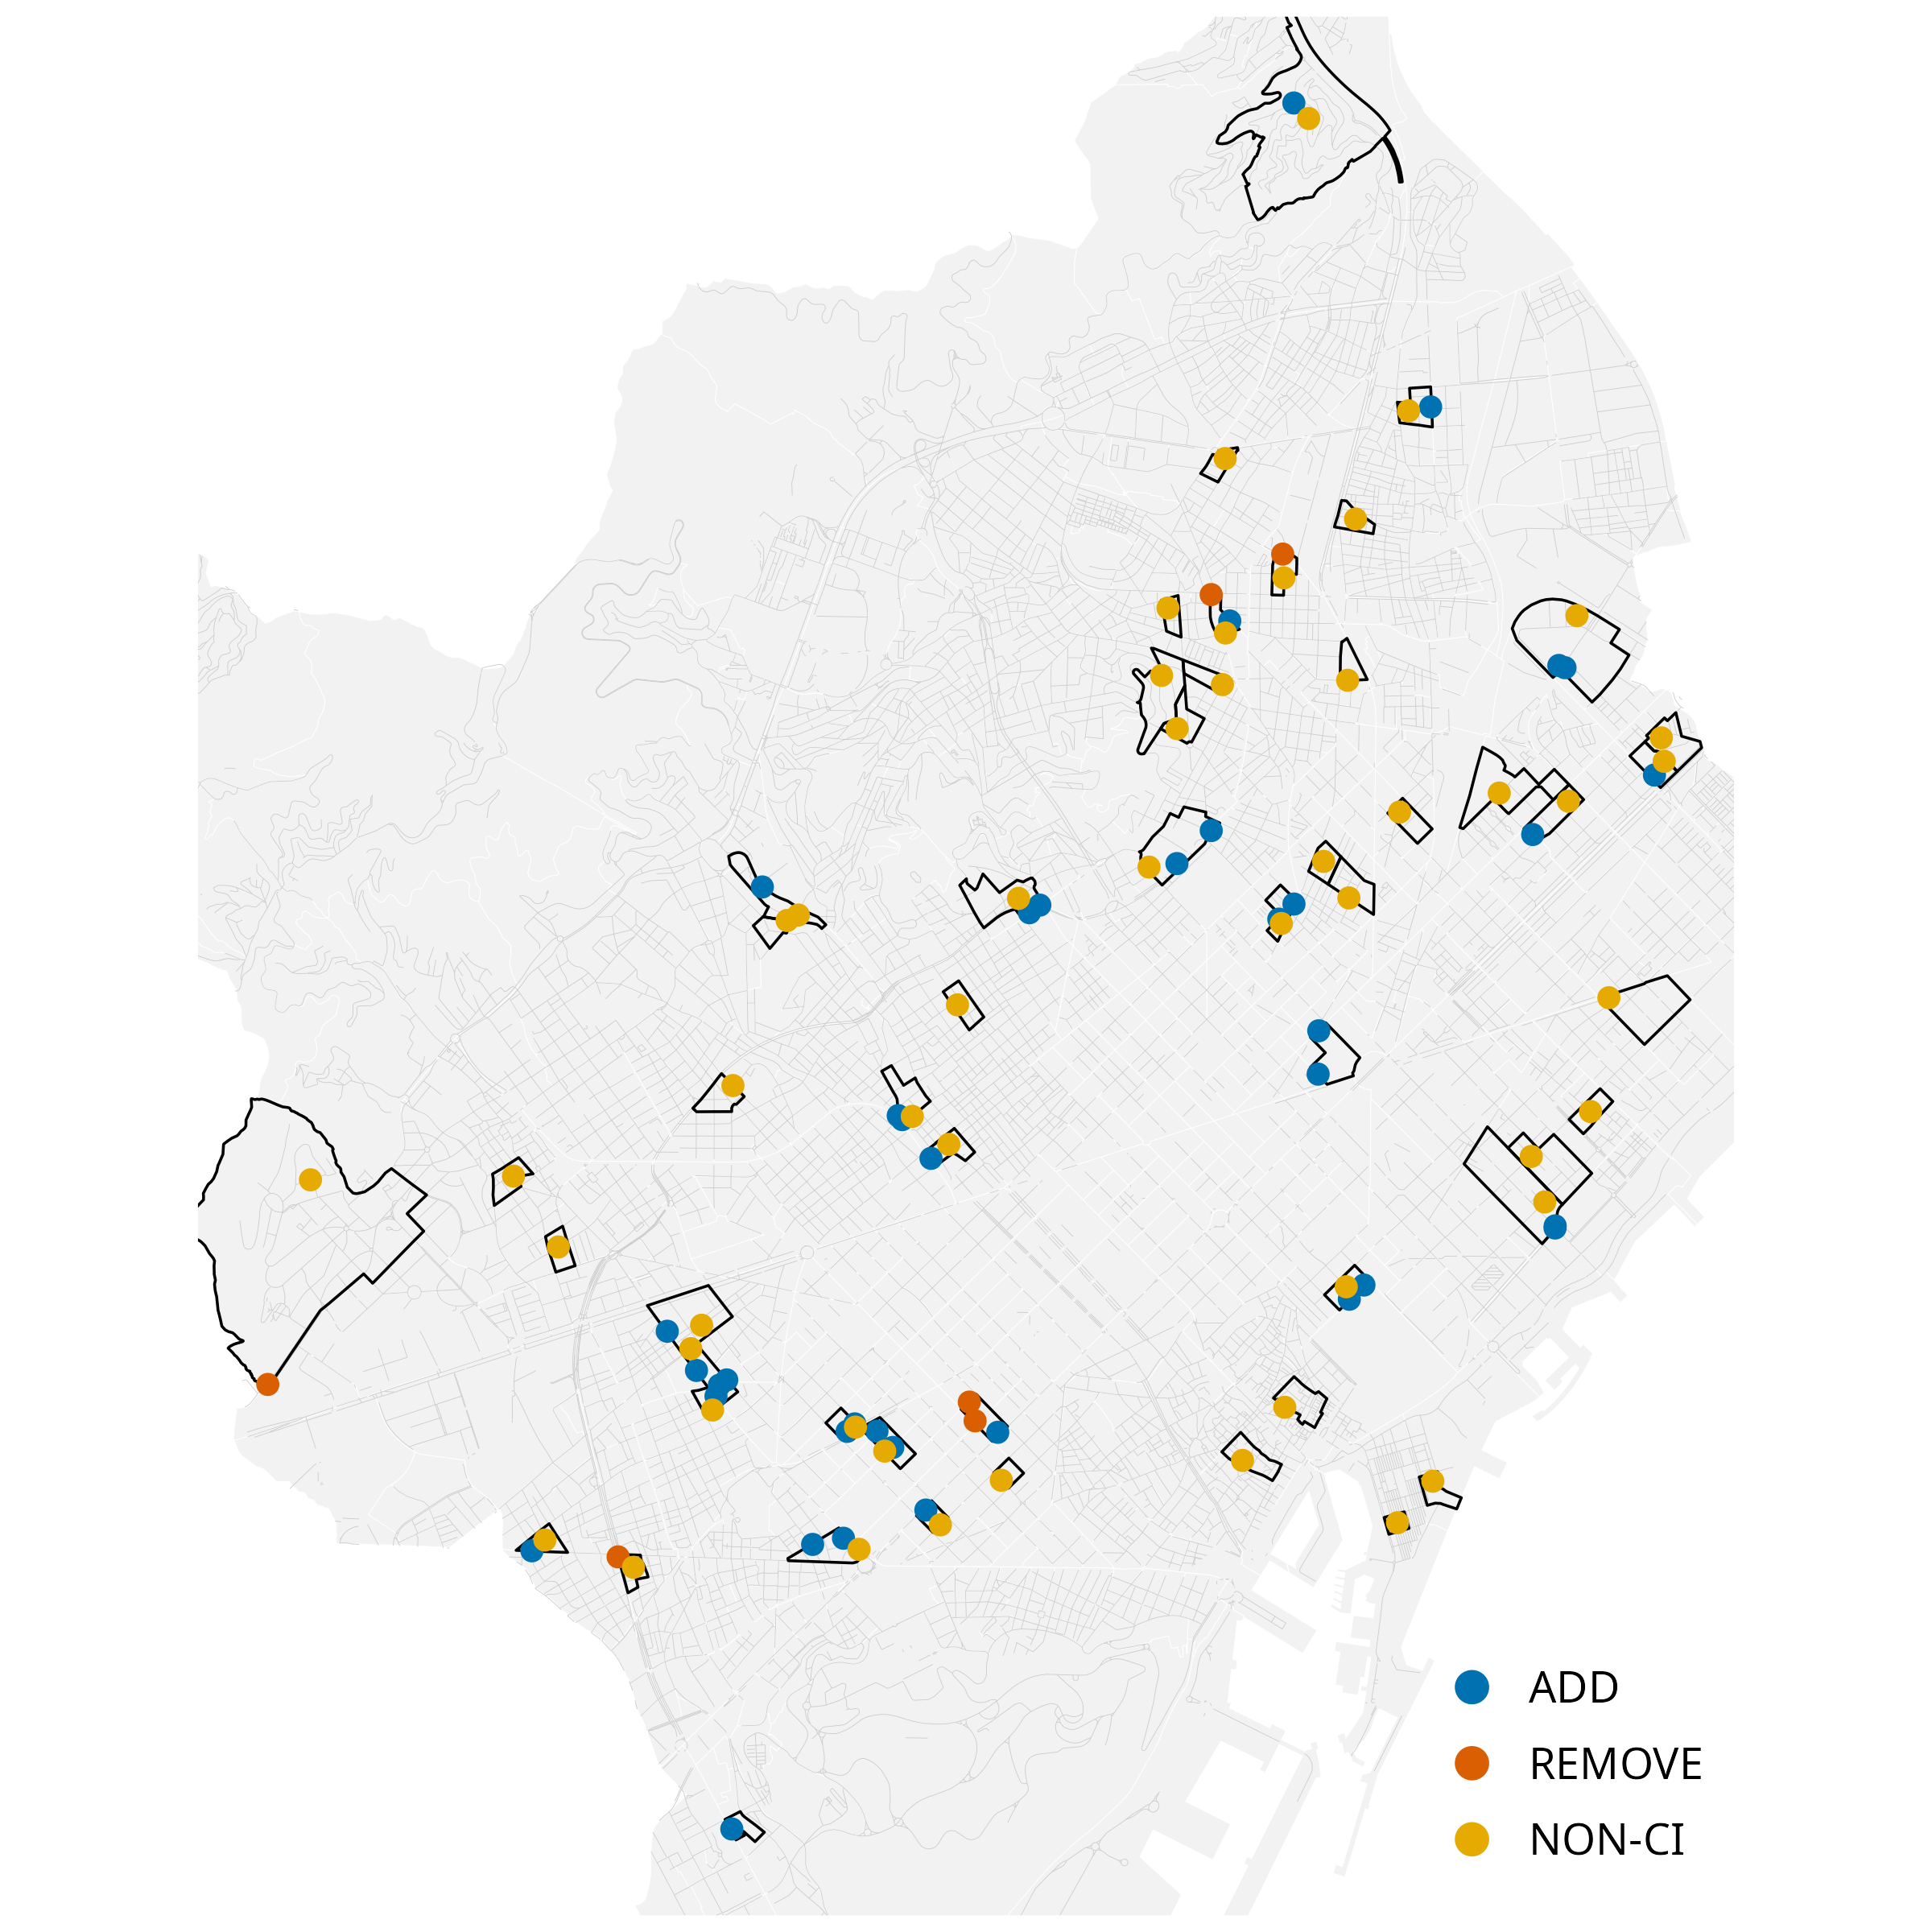
\includegraphics[width=1\linewidth,height=\textheight,keepaspectratio]{../figs/validation_points_map.png}

}

\subcaption{\label{fig-strata-validation-2}}

\end{minipage}%

\caption{\label{fig-strata-validation}Outputs used in the validation
design: (a) Bivariate tract stratification; (b) Validation points by
type.}

\end{figure}%

\textbf{Step 4. Inspect and code GSV}

Each validation site was independently coded by two trained coders
following a standardised protocol (Supplement
\hyperref[s3-gsv-protocol]{S3}). Coders assessed whether cycling
infrastructure was present in a baseline and follow-up period
corresponding to the OSM reference snapshots. When the nearest panorama
did not provide a clear view of the sampled location, coders were
permitted to adjust the Street View position slightly along the same
street segment, provided that the original sampled point remained
visible and spatially identifiable. For each site and period, coders
recorded infrastructure presence/absence and the month of the imagery
used.

Because GSV imagery availability varies across locations and years,
coders prioritised imagery as close as possible to the reference dates.
For the baseline period, coders attempted 2016 and 2015 first (using
2014 only as a fallback when required); for the follow-up period, coders
attempted 2024 and 2023 first (using 2022 only as a fallback when
required). When multiple candidate years were available, the observation
closest in time to the reference date was selected to define adjudicated
baseline and follow-up values.

Sites were coded as missing when available imagery did not allow a clear
determination of cycling-infrastructure presence for the reference
period (e.g., obscured views, roadworks, or ambiguous visual evidence).
Missing observations were excluded from accuracy analyses requiring
adjudicated baseline and follow-up values. Intercoder agreement was
assessed on usable sites, and any discrepancies were resolved through
reconciliation to produce a final adjudicated dataset for analysis.

\textbf{Step 5. Evaluate OSM performance}

Using the adjudicated baseline and follow-up GSV codes, we evaluated
whether OSM snapshot differencing correctly identified additions and
removals of cycling infrastructure. For segments flagged as additions, a
true positive (TP) corresponded to a 0→1 transition between baseline and
follow-up, whereas a false positive (FP) corresponded to no change (0→0)
or persistence of cycling infrastructure (1→1). For segments flagged as
removals, a TP corresponded to a 1→0 transition, whereas an FP
corresponded to no change (1→1) or no cycling infrastructure in either
period (0→0). NONCYC control locations were used to identify false
negatives (FN), defined as cycling-infrastructure changes visible in GSV
but not detected by OSM differencing. Examples of TP additions and
removals are shown in Figure~\ref{fig-gsv-examples}.

\begin{figure}[htbp]

\begin{minipage}{0.50\linewidth}

\centering{

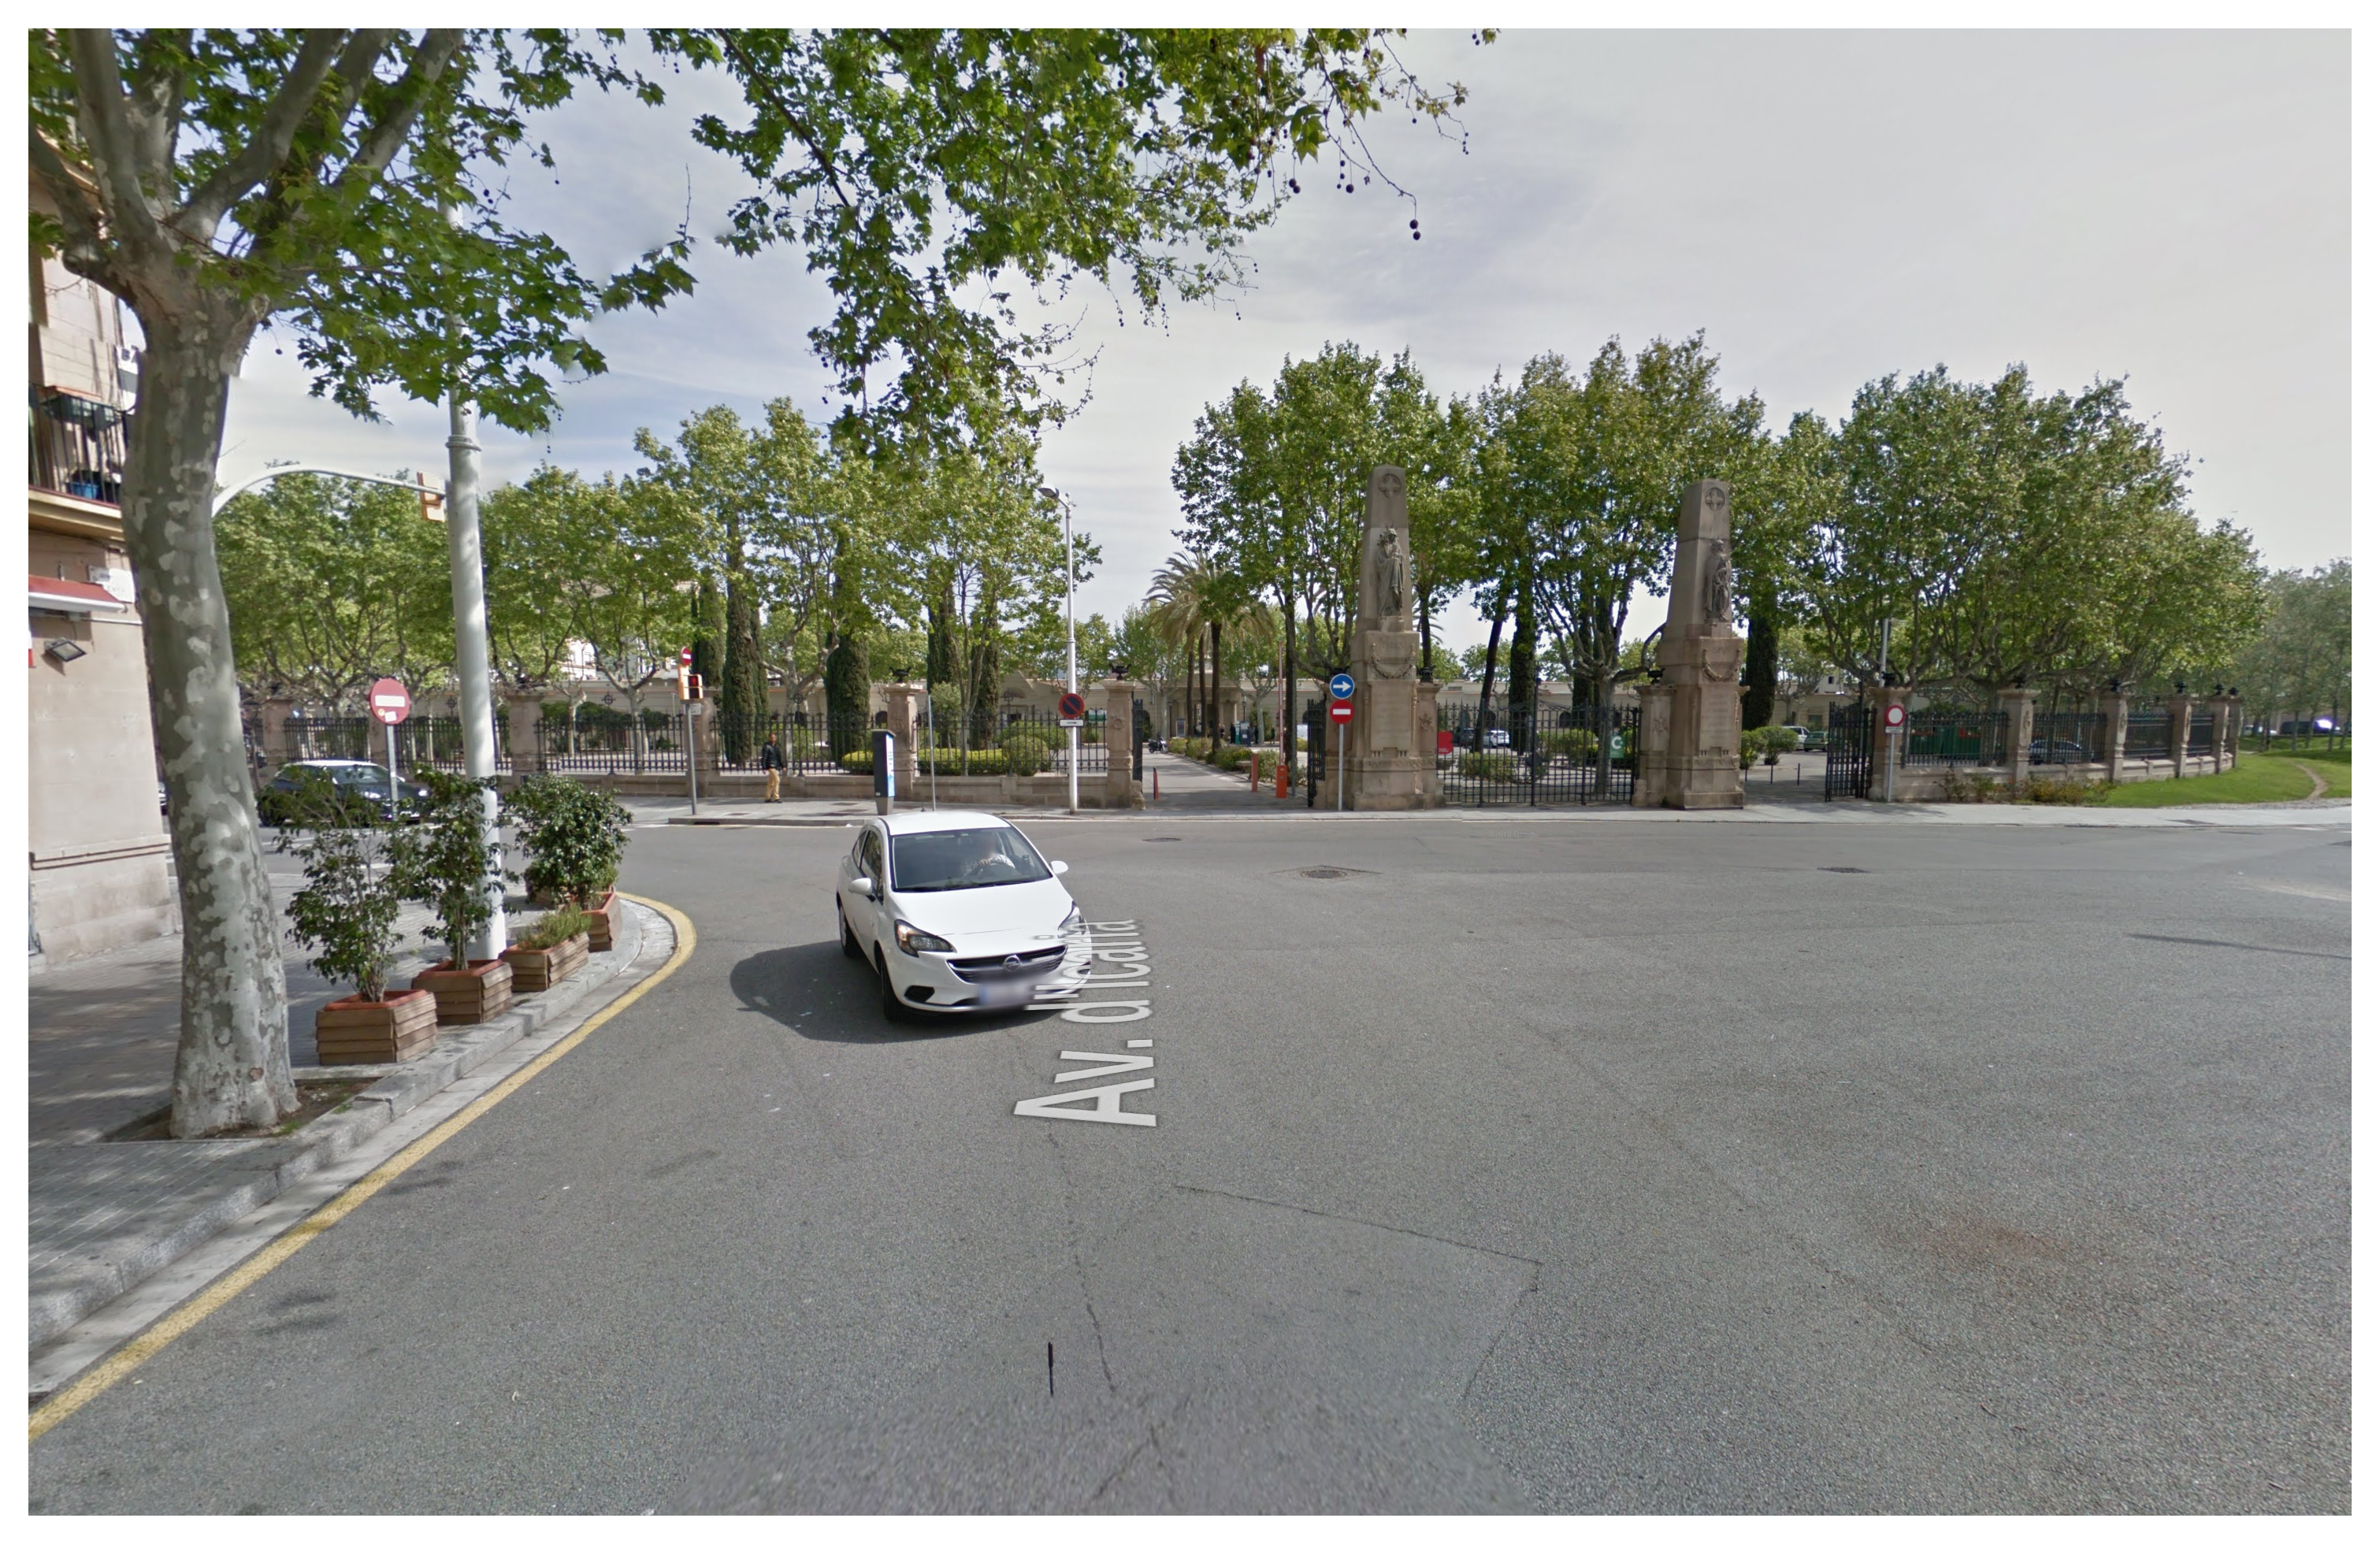
\includegraphics[width=1\linewidth,height=\textheight,keepaspectratio]{../figs/_framed/addition-2015.png}

}

\subcaption{\label{fig-gsv-examples-1}}

\end{minipage}%
%
\begin{minipage}{0.50\linewidth}

\centering{

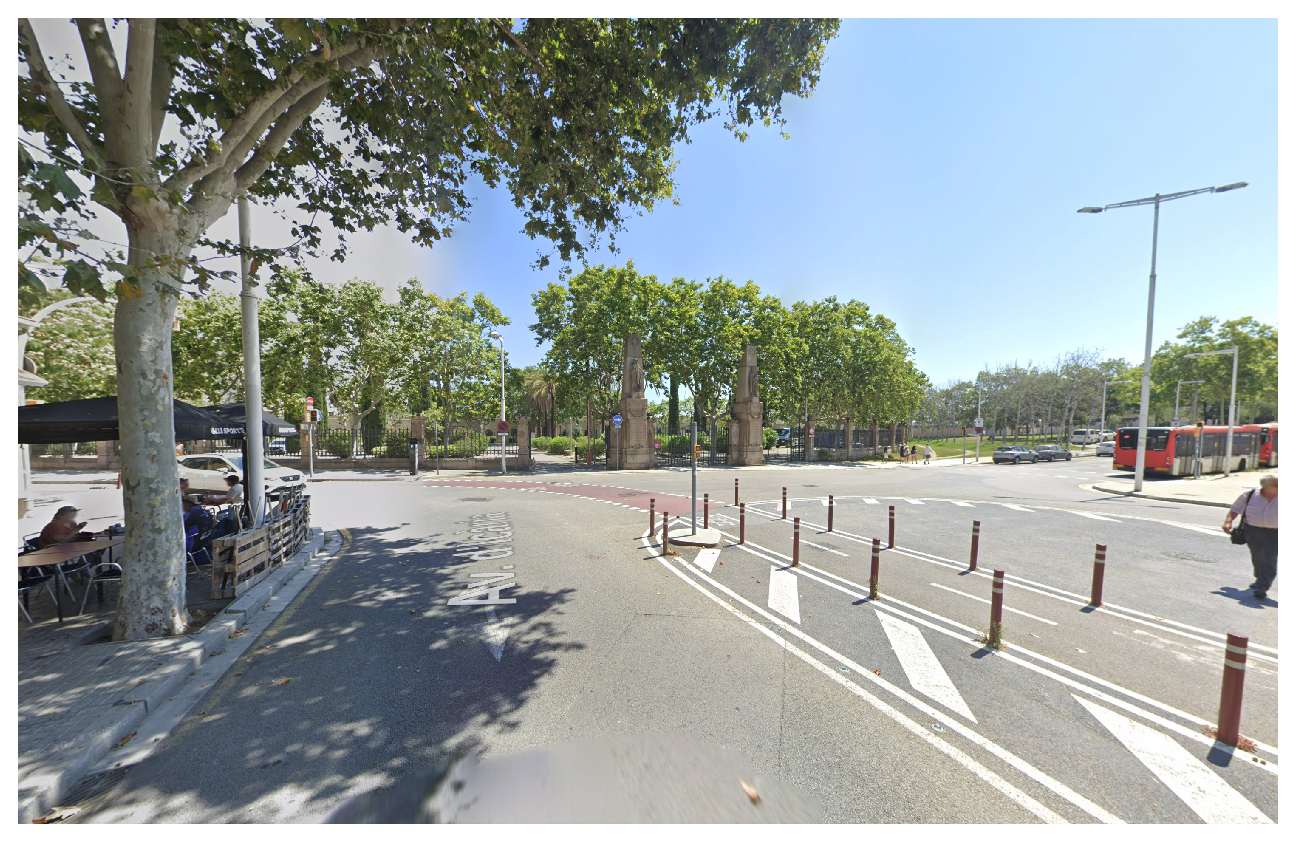
\includegraphics[width=1\linewidth,height=\textheight,keepaspectratio]{../figs/_framed/addition-2023.png}

}

\subcaption{\label{fig-gsv-examples-2}}

\end{minipage}%
\newline
\begin{minipage}{0.50\linewidth}

\centering{

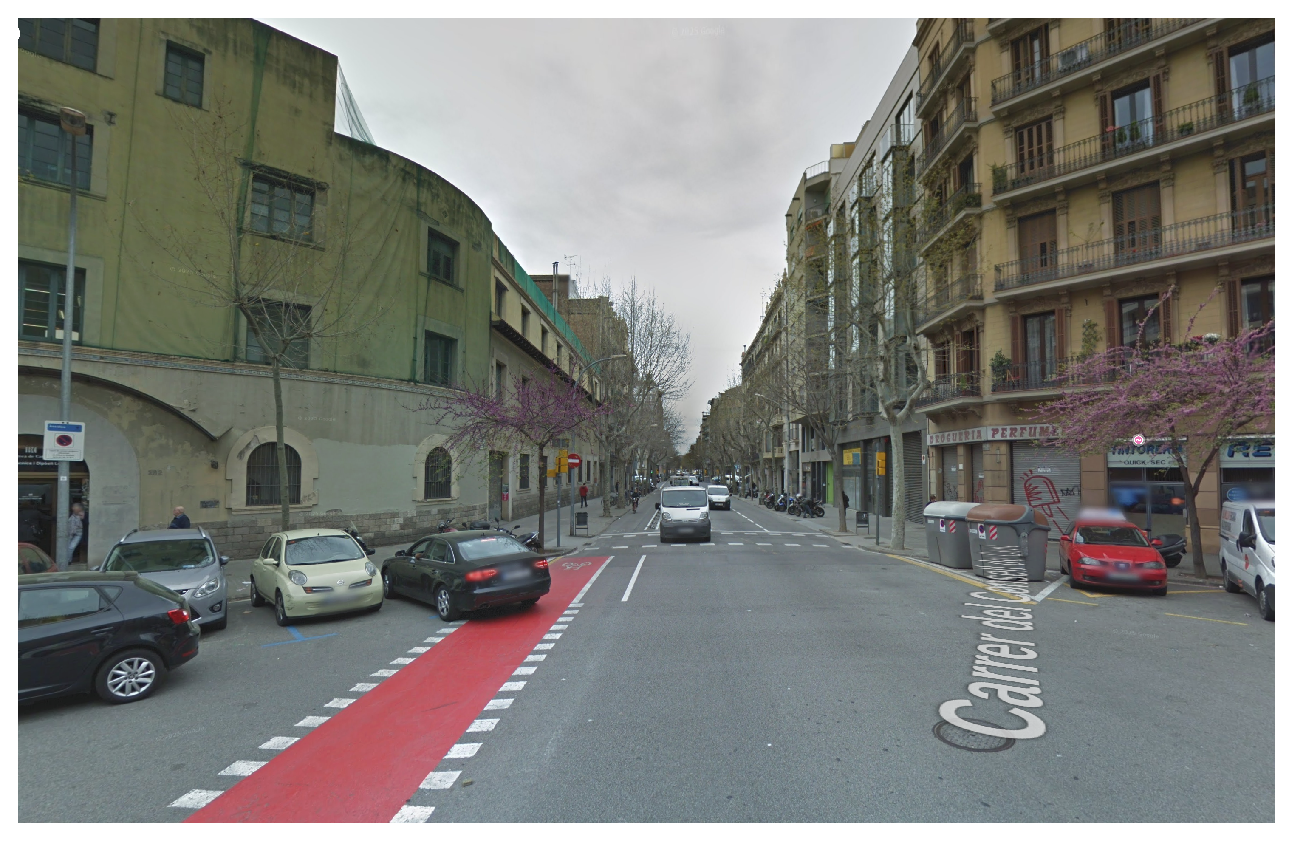
\includegraphics[width=1\linewidth,height=\textheight,keepaspectratio]{../figs/_framed/removal-2015.png}

}

\subcaption{\label{fig-gsv-examples-3}}

\end{minipage}%
%
\begin{minipage}{0.50\linewidth}

\centering{

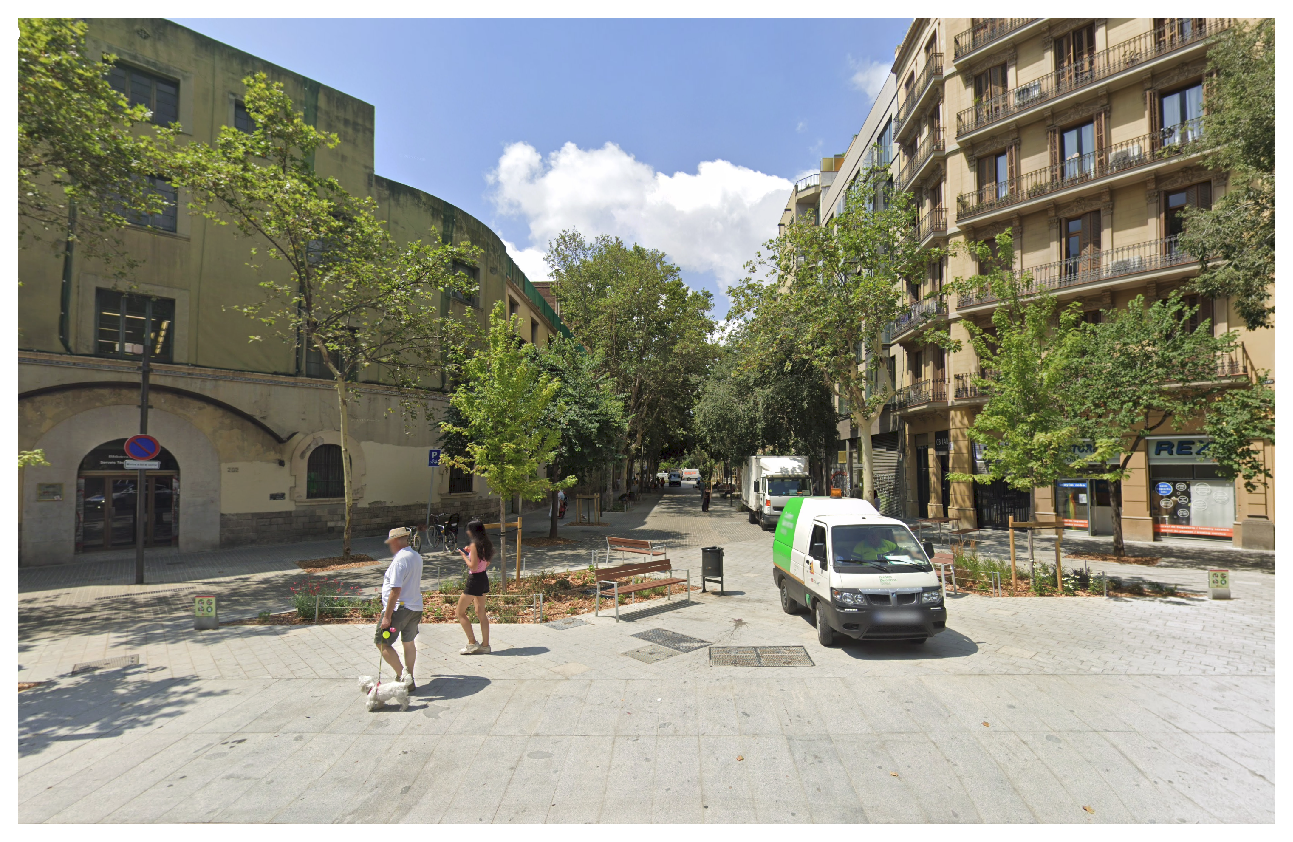
\includegraphics[width=1\linewidth,height=\textheight,keepaspectratio]{../figs/_framed/removal-2023.png}

}

\subcaption{\label{fig-gsv-examples-4}}

\end{minipage}%

\caption{\label{fig-gsv-examples}Examples of true positive changes
identified during GSV validation: (a) 2015 baseline without cycling
infrastructure; (b) 2023 follow-up showing a newly implemented
segregated cycle track (0 → 1); (c) 2015 baseline with a cycle track;
(d) 2023 follow-up showing its removal following street redesign (1 →
0).}

\end{figure}%

Validation performance was summarised using standard classification
metrics based on the final reconciled validation dataset (Supplement
\hyperref[s4-joined-results]{S4}). Precision, recall and the F1 score
were computed as:

\[
\text{Precision}=\frac{TP}{TP+FP},\quad
\text{Recall}=\frac{TP}{TP+FN},\quad
F_1=\frac{2\cdot \text{Precision}\cdot \text{Recall}}{\text{Precision}+\text{Recall}}.
\] Pooled metrics were computed by first aggregating TP, FP and FN
across addition and removal events, and then calculating precision,
recall and the F1 score from these pooled counts. For precision and
recall, 95\% confidence intervals were computed using Wilson score
intervals for the corresponding numerators and denominators, which
provide stable coverage for proportions, particularly with small sample
sizes or extreme values.

All data processing, change detection, sampling, and validation
procedures were implemented in an open-source R workflow. Code
availability is detailed in the \hyperref[s1-code]{Data and code
availability} section.

\section{Results}\label{results}

\subsection{Network change detected from OSM
(2015--2023)}\label{network-change-detected-from-osm-20152023}

Between 2015 and 2023, the OSM-derived cycling network in Barcelona
increased from 130.7 to 235.7 km, corresponding to a net growth of 105.0
km, an 80.3 \% increase (Figure~\ref{fig-changes}). Network lengths were
calculated as the summed length of cycling-infrastructure line
geometries in OSM, without collapsing parallel or spatially separated
facilities into a single corridor-level measure (e.g., cycle tracks on
both sides of a street). Geometric differencing identified 127.1 km of
added and 24.9 km of removed cycling infrastructure, yielding a net
change of 102.2 km. The small discrepancy (−2.8 km) reflects minor
geometric artefacts introduced by the buffering, dissolving, and
fragment-filtering steps used in the differencing procedure, and
indicates good internal consistency between aggregate network totals and
change estimates (Table~\ref{tbl-consistency}).

\begin{longtable}[]{@{}lr@{}}

\caption{\label{tbl-consistency}Consistency between yearly totals and
differencing estimates (2015--2023, Barcelona)}

\tabularnewline

\toprule\noalign{}
Metric & Value (km) \\
\midrule\noalign{}
\endhead
\bottomrule\noalign{}
\endlastfoot
Total network length (2015) & 130.7 \\
Total network length (2023) & 235.7 \\
Net growth (2023 − 2015) & 105.0 \\
Additions & 127.1 \\
Removals & 24.9 \\
Additions − removals & 102.2 \\
Gap: (Additions − removals) − Net & -2.8 \\

\end{longtable}

OSM-detected additions were unevenly distributed across the city.
Low-density strata (D1\_C1, D1\_C2 and D1\_C3) accounted for 60.0 \% of
all added length, with particularly large gains in low-density
peripheral (D1\_C1) and low-density central (D1\_C3) areas
(Table~\ref{tbl-distribution-strata}). Additions were also substantial
in medium-density central tracts (D2\_C3) and high-density central
tracts (D3\_C3), indicating that expansion was not confined to the urban
periphery. In contrast, removals were limited in total length and were
more unevenly distributed, with the largest shares observed in
low-density central areas (D1\_C3; 37.7 \%) and low-density peripheral
areas (D1\_C1; 28.8 \%), while all other strata each accounted for less
than 12 \% of removed length.

\begin{longtable}[]{@{}
  >{\raggedright\arraybackslash}p{(\linewidth - 10\tabcolsep) * \real{0.0964}}
  >{\raggedright\arraybackslash}p{(\linewidth - 10\tabcolsep) * \real{0.3494}}
  >{\raggedleft\arraybackslash}p{(\linewidth - 10\tabcolsep) * \real{0.1325}}
  >{\raggedleft\arraybackslash}p{(\linewidth - 10\tabcolsep) * \real{0.1566}}
  >{\raggedleft\arraybackslash}p{(\linewidth - 10\tabcolsep) * \real{0.1205}}
  >{\raggedleft\arraybackslash}p{(\linewidth - 10\tabcolsep) * \real{0.1446}}@{}}

\caption{\label{tbl-distribution-strata}OSM-estimated additions and
removals (2015--2023) by density × centrality stratum. Totals may differ
slightly from the aggregate city-level estimates because change segments
are split at census-tract boundaries before aggregation.}

\tabularnewline

\toprule\noalign{}
\begin{minipage}[b]{\linewidth}\raggedright
Stratum
\end{minipage} & \begin{minipage}[b]{\linewidth}\raggedright
Definition
\end{minipage} & \begin{minipage}[b]{\linewidth}\raggedleft
Added (km)
\end{minipage} & \begin{minipage}[b]{\linewidth}\raggedleft
Removed (km)
\end{minipage} & \begin{minipage}[b]{\linewidth}\raggedleft
Added (\%)
\end{minipage} & \begin{minipage}[b]{\linewidth}\raggedleft
Removed (\%)
\end{minipage} \\
\midrule\noalign{}
\endhead
\bottomrule\noalign{}
\endlastfoot
D1\_C1 & Low density, peripheral & 31.0 & 7.0 & 24 & 29 \\
D1\_C2 & Low density, intermediate & 16.0 & 1.0 & 13 & 4 \\
D1\_C3 & Low density, central & 29.0 & 9.0 & 23 & 38 \\
D2\_C1 & Medium density, peripheral & 2.0 & 0.0 & 2 & 2 \\
D2\_C2 & Medium density, intermediate & 11.0 & 1.0 & 9 & 6 \\
D2\_C3 & Medium density, central & 15.0 & 3.0 & 12 & 11 \\
D3\_C1 & High density, peripheral & 1.0 & 0.0 & 1 & 0 \\
D3\_C2 & High density, intermediate & 10.0 & 1.0 & 8 & 5 \\
D3\_C3 & High density, central & 12.0 & 1.0 & 9 & 5 \\
TOTAL & All strata combined & 126.8 & 24.8 & 100 & 100 \\

\end{longtable}

\begin{figure}

\centering{

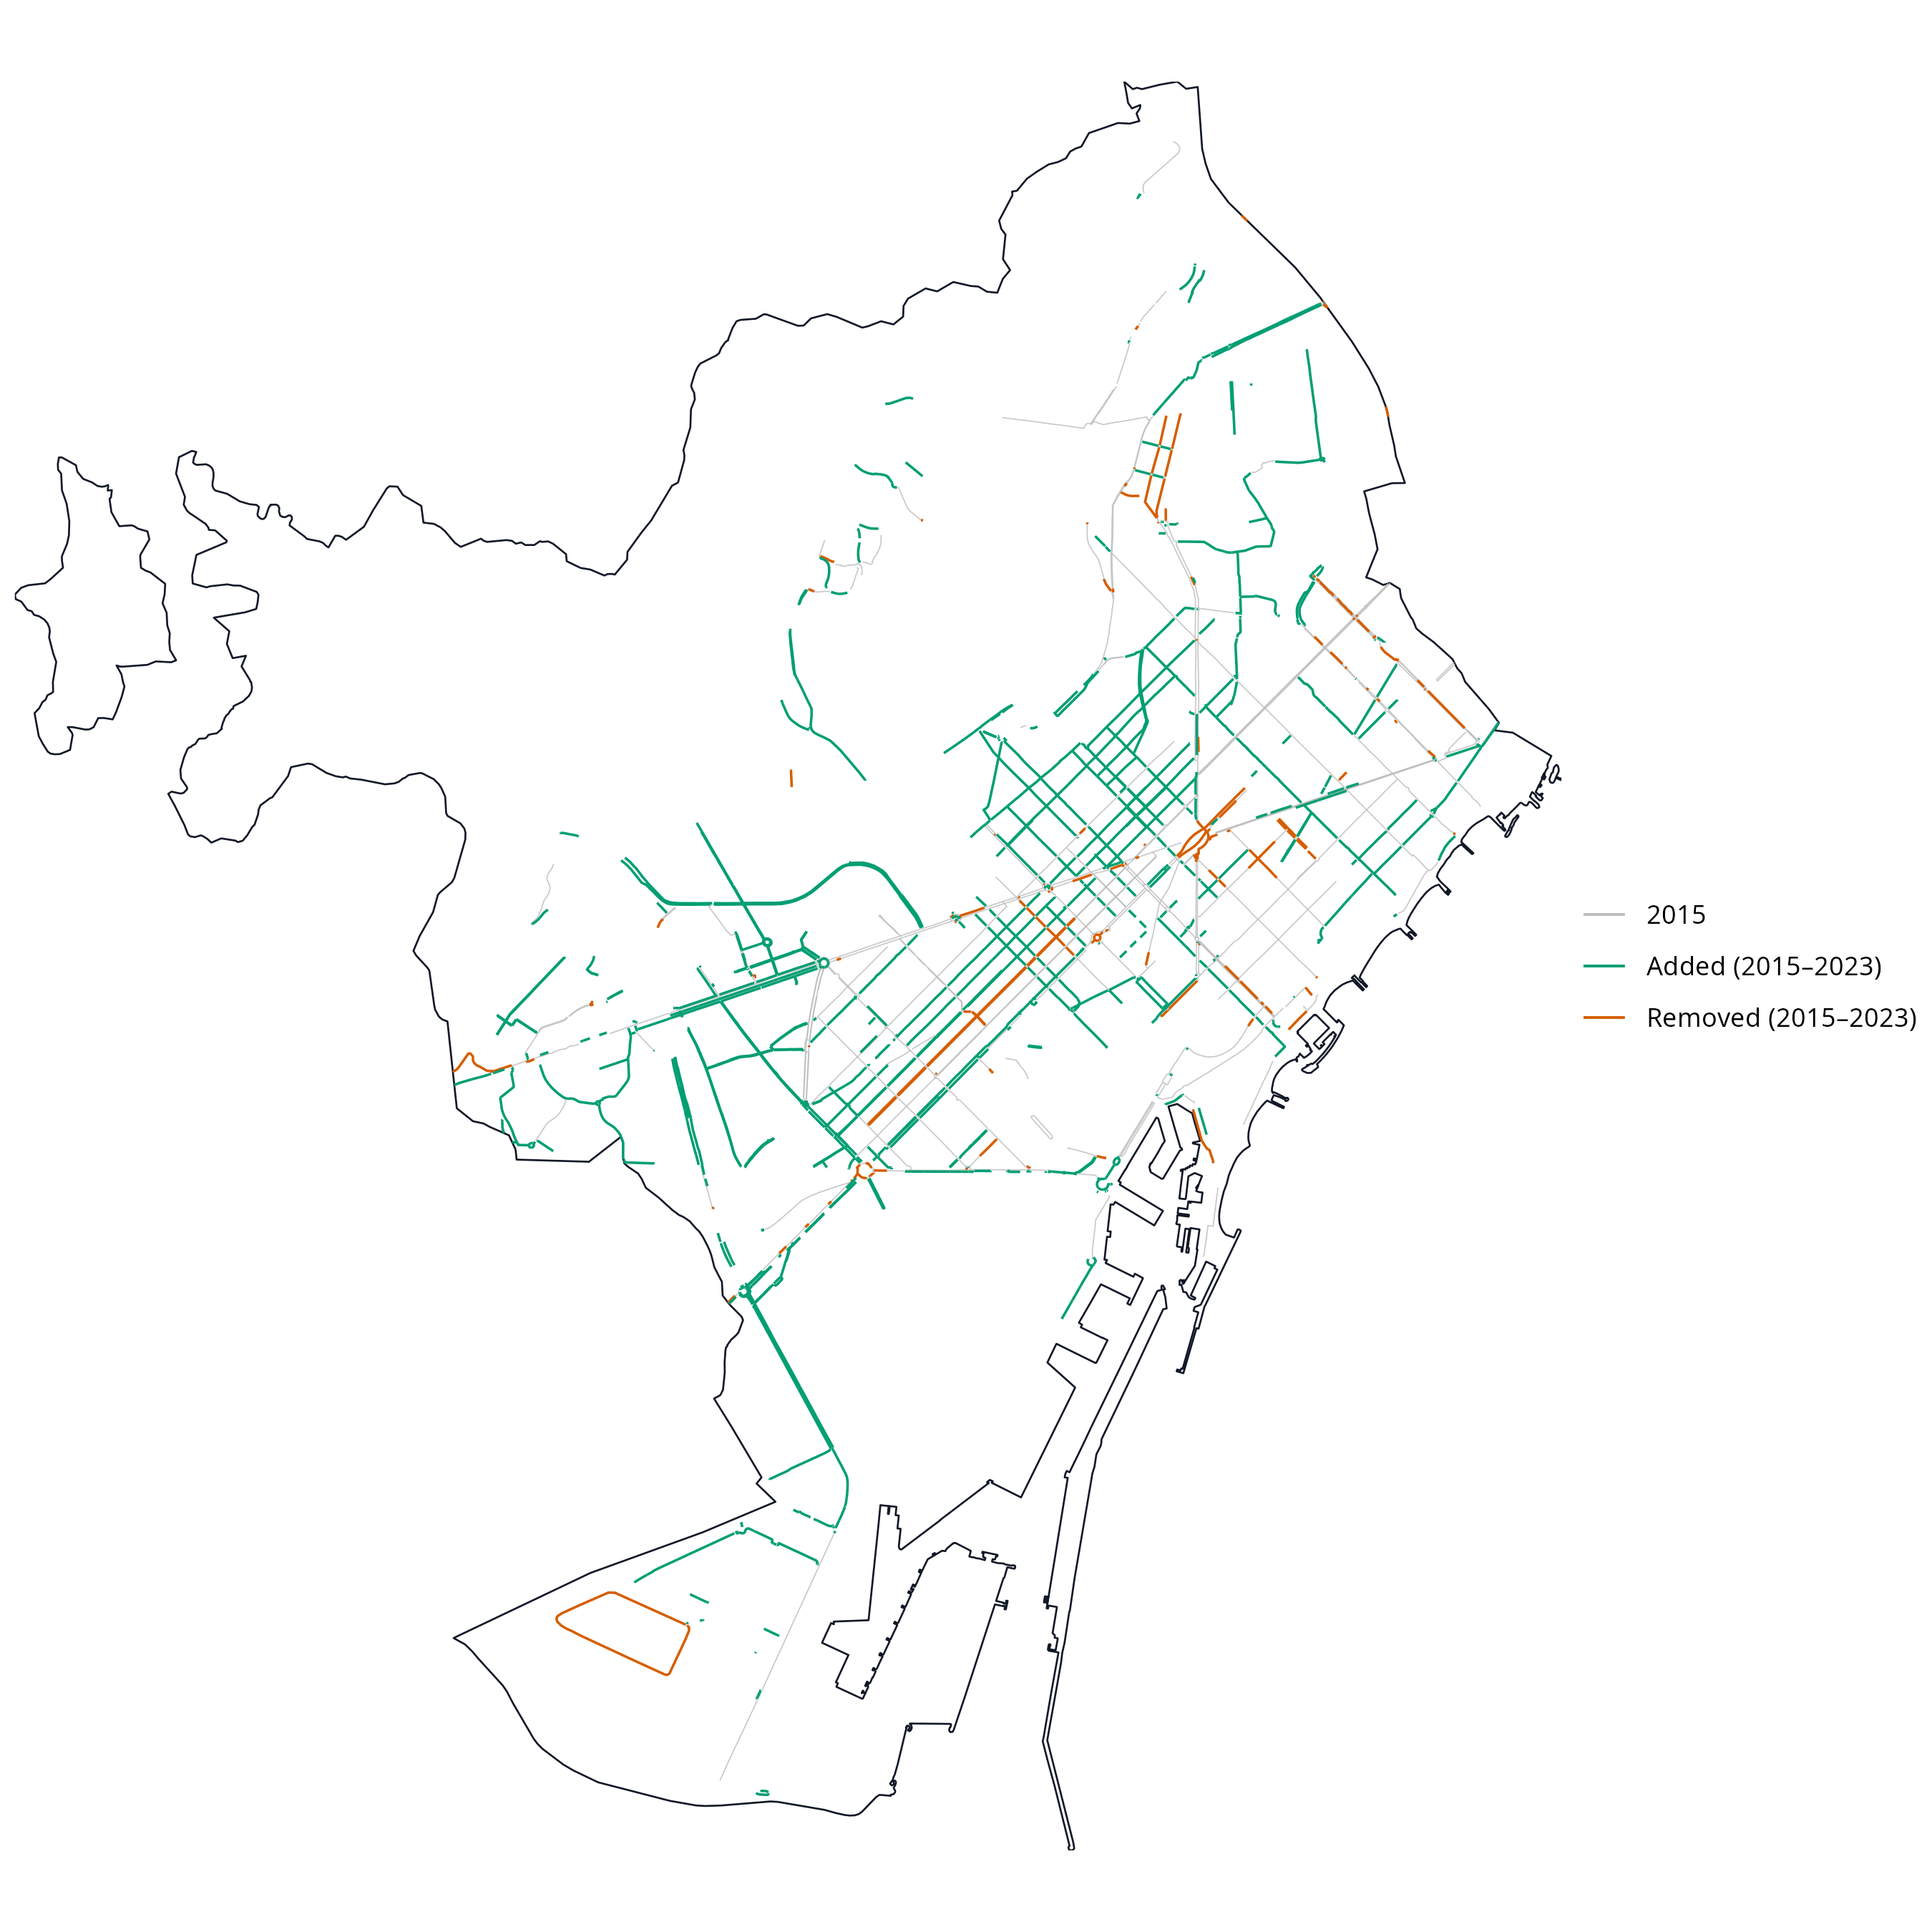
\includegraphics[width=1\linewidth,height=\textheight,keepaspectratio]{../figs/infra_change_map.png}

}

\caption{\label{fig-changes}OSM-detected cycling-infrastructure changes
in Barcelona, 2015--2023.}

\end{figure}%

\subsection{Validation of OSM-detected changes using
GSV}\label{validation-of-osm-detected-changes-using-gsv}

Of the 105 sampled sites (39 additions, 6 removals and 50 non-cycling
control sites), 86 (82\%) provided usable GSV panoramas for both the
baseline and follow-up periods, yielding 33 additions, 5 removals and 48
non-cycling control sites for analysis
(Table~\ref{tbl-summary_stratum}). These validation points were
distributed across all density--centrality strata, reflecting the
stratified sampling design and the spatial availability of candidate
change segments within the sampled tracts.

\begin{longtable}[]{@{}llrrrr@{}}

\caption{\label{tbl-summary_stratum}Validation points by class and
stratum (usable points only)}

\tabularnewline

\toprule\noalign{}
Stratum & Definition & Add & Remove & NONCYC & Total \\
\midrule\noalign{}
\endhead
\bottomrule\noalign{}
\endlastfoot
D1\_C1 & Low density, peripheral & 5 & 1 & 6 & 12 \\
D1\_C2 & Low density, intermediate & 5 & 0 & 4 & 9 \\
D1\_C3 & Low density, central & 6 & 0 & 5 & 11 \\
D2\_C1 & Medium density, peripheral & 2 & 2 & 6 & 10 \\
D2\_C2 & Medium density, intermediate & 4 & 0 & 6 & 10 \\
D2\_C3 & Medium density, central & 3 & 1 & 5 & 9 \\
D3\_C1 & High density, peripheral & 1 & 0 & 6 & 7 \\
D3\_C2 & High density, intermediate & 3 & 1 & 5 & 9 \\
D3\_C3 & High density, central & 4 & 0 & 5 & 9 \\
TOTAL & All strata combined & 33 & 5 & 48 & 86 \\

\end{longtable}

Initial intercoder agreement on the binary presence/absence coding was
92\% (79/86). The remaining 7 cases were resolved by consensus, and the
adjudicated baseline and follow-up values were used in the accuracy
analysis.

Table~\ref{tbl-validation} summarises the validation outcomes, and
Figure~\ref{fig-validation-metrics} provides a visual comparison of
precision and recall with 95\% CI across change classes. CI reflect
sampling uncertainty in the GSV validation and are wider for classes
with fewer usable sites. For additions, OSM shows high recall (0.96, 95
\% CI {[}0.82--0.99{]}) and good precision (0.82, 95 \% CI
{[}0.66--0.91{]}), indicating that most real additions were detected,
although some false positives remain. For removals, recall is 1.00 but
with a very wide confidence interval due to the small sample size (n =
5), while precision is very poor (0.20, 95 \% CI {[}0.04--0.62{]}),
suggesting that most OSM-detected removals do not correspond to true
infrastructure loss. When pooling additions and removals, overall
precision is 0.74, recall is 0.97, and the F1 score is 0.84, reflecting
strong sensitivity to change but more limited specificity, particularly
for removals.

\begin{longtable}[t]{>{\raggedright\arraybackslash}p{2 cm}rrrrrrr}

\caption{\label{tbl-validation}Validation metrics for OSM inferred
cycling-infrastructure changes (2015--2023). ``ADD'' refers to added
segments (present in 2023 but not in 2015); ``REMOVE'' refers to removed
segments (present in 2015 but not in 2023); ``Pooled'' combines both
change types. ``n (usable)'' is the number of sampled segments with
codable GSV panoramas for both years. Precision and recall 95\%
confidence intervals are Wilson score intervals.}

\tabularnewline

\toprule
Class & n (usable) & TP & FP & FN & Precision (95\% CI) & Recall (95\% CI) & F1\\
\midrule
ADD & 33 & 27 & 6 & 1 & 0.82 [0.66-0.91] & 0.96 [0.82-0.99] & 0.89\\
REMOVE & 5 & 1 & 4 & 0 & 0.20 [0.04-0.62] & 1.00 [0.21-1.00] & 0.33\\
Pooled & 38 & 28 & 10 & 1 & 0.74 [0.58-0.85] & 0.97 [0.83-0.99] & 0.84\\
\bottomrule

\end{longtable}

\begin{figure}

\centering{

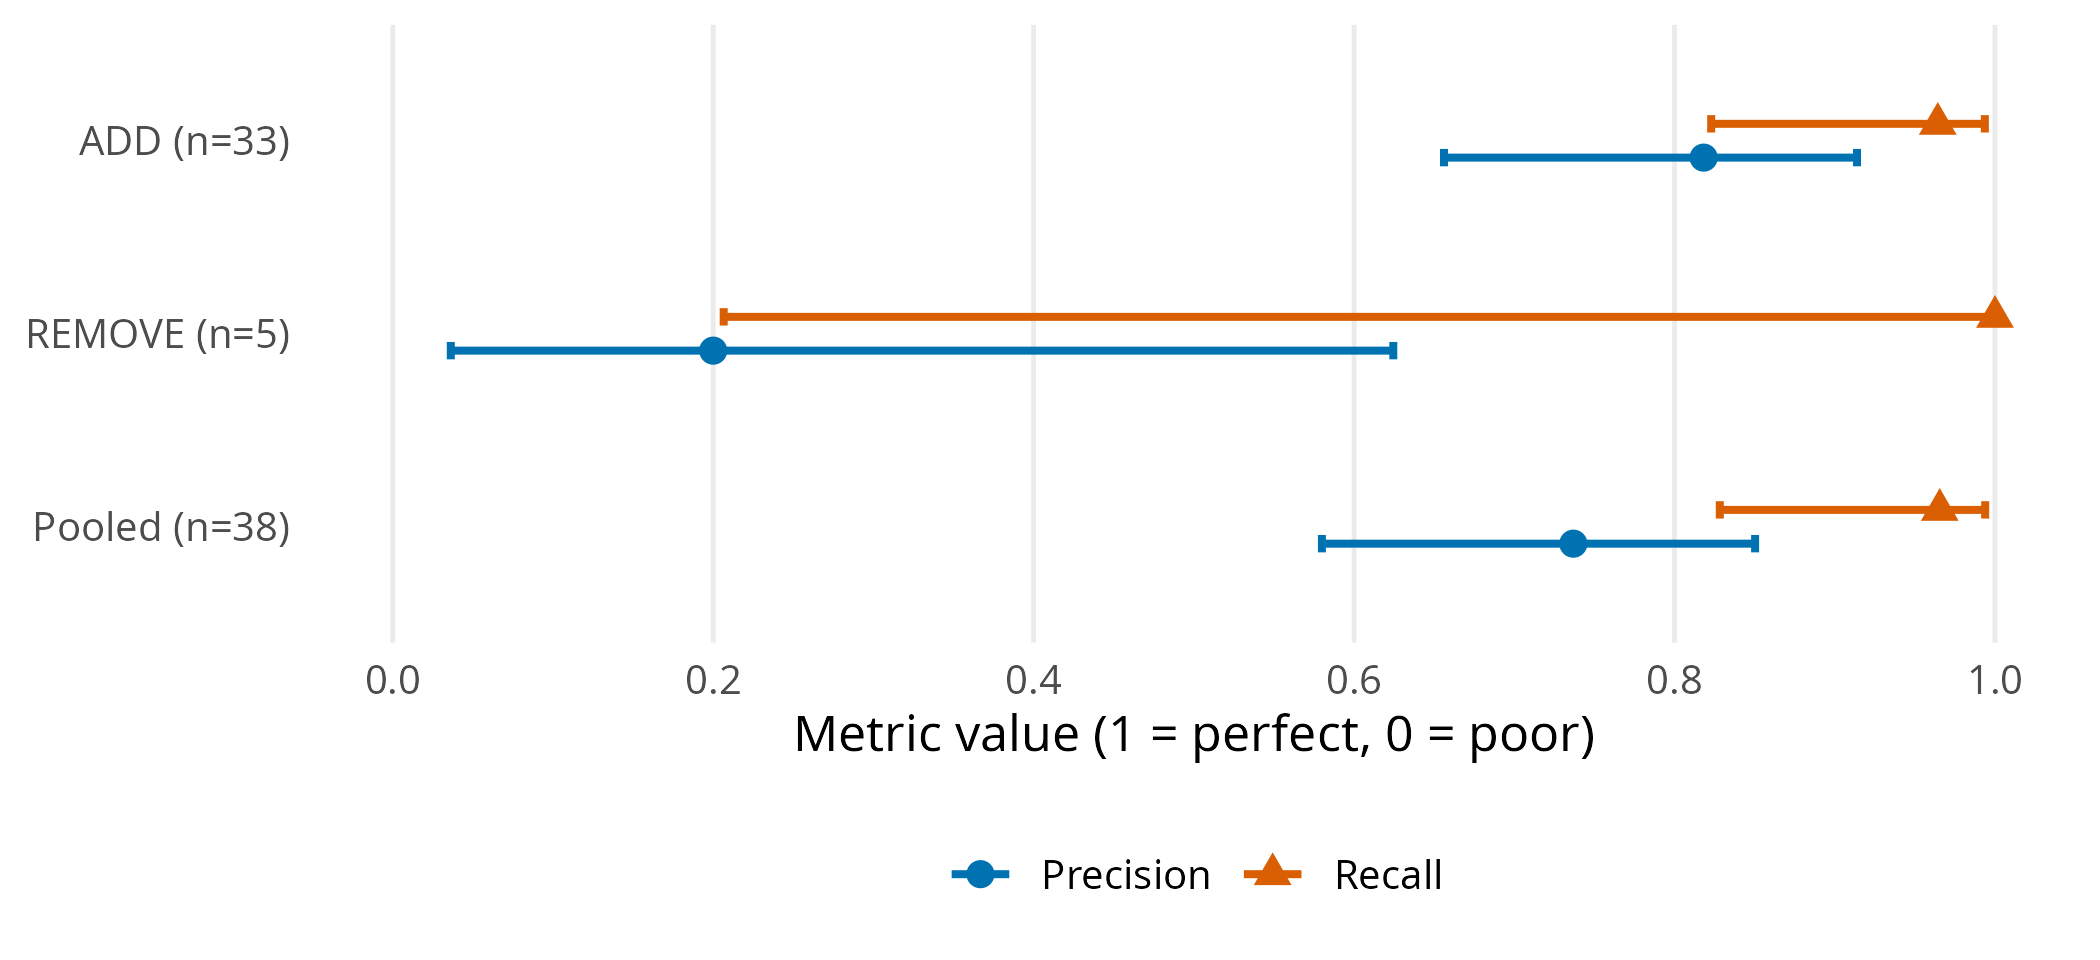
\includegraphics[width=0.9\linewidth,height=\textheight,keepaspectratio]{../figs/validation-metrics.png}

}

\caption{\label{fig-validation-metrics}Precision and recall (with 95\%
confidence intervals) for OSM-inferred cycling-infrastructure changes.}

\end{figure}%

\section{Discussion}\label{discussion}

This study quantified the temporal accuracy of OSM-derived
cycling-infrastructure change in Barcelona (2015--2023) by combining
longitudinal snapshot differencing with stratified GSV validation. To
date, the available literature has either validated OSM cycling
infrastructure cross-sectionally against reference datasets (Ferster et
al. 2020; Hochmair, Zielstra, and Neis 2015), used OSM snapshots to
measure cycling-network growth at scale without externally validating
whether detected changes reflect on-street infrastructure change
(Winters, Ferster, and Laberee 2025), or applied street-level imagery to
audit built-environment features independently of OSM (Rundle et al.
2011). By designing and implementing a transparent end-to-end workflow
combining historical network reconstruction, geometric differencing,
stratified spatial sampling, and independent visual verification, we
produce reproducible, transferable accuracy metrics (including
precision, recall, and F1 score) for cycling-infrastructure change
detection. Our workflow therefore provides a practical calibration
strategy for longitudinal research using OSM when authoritative
year-on-year inventories are unavailable.

Overall, OSM performed well in detecting cycling-infrastructure
additions, but performance was substantially weaker for removals.
Although recall remained high for both change types, precision for
removals was very low, indicating that most apparent removals detected
through snapshot differencing do not correspond to actual on-street
cycling-infrastructure loss. These results highlight that OSM-derived
removals must be carefully verified before estimating net changes in the
cycling network.

To understand this asymmetry, it is important to consider how OSM
records change over time. Because OSM objects can be split, merged,
re-tagged, deleted, or recreated (Minghini and Frassinelli 2019),
structural edits between snapshots may produce apparent removals without
corresponding physical change on the street. This is especially likely
for removals, as segments may disappear from a snapshot when they are
re-drawn with new geometries, reclassified under different tags, or
merged into adjacent features, even though the underlying infrastructure
remains in place. Additions, in contrast, require the introduction of
new geometries or tags and may therefore more often correspond to
genuinely new on-street features. OSM-based differencing can therefore
over-detect removals when edits reflect changes in representation rather
than physical interventions. This is consistent with the nature of OSM
as a continuously edited VGI resource, in which objects are routinely
revised rather than fixed as in a static dataset (Goodchild 2007).

From a practical perspective, for cities that lack consistently
maintained inventories, OSM snapshot differencing can function as a
screening tool for identifying likely infrastructure additions at scale,
with targeted imagery checks providing an efficient quality-control
layer. This matters because practitioners often need to monitor delivery
(corridor completion, network coverage growth) and to allocate limited
auditing resources; virtual audits have repeatedly been shown to reduce
the burden of in-person observation while remaining usable for
built-environment measurement (Rundle et al. 2011). Our results suggest
that OSM-derived additions can be treated as generally informative, but
apparent removals should not be interpreted as ``rollback'' without
independent verification.

Beyond planning practice, these measurement characteristics also have
implications for longitudinal research designs. Studies evaluating
cycling interventions often rely on the timing and location of network
changes to define exposure, treatment, and control conditions at the
street or neighborhood level. When removals are over-detected, analyses
can be substantially distorted, and even net growth can be biased in
settings where apparent removals are more frequent than in Barcelona.
More importantly, misclassifying segments as removed could bias
estimates in longitudinal designs that depend on staggered
implementation and upgrades. In this context, the observed precision
values can be used to inform calibration of snapshot-differenced
estimates. For example, scaling raw OSM change counts by change-specific
precision (approximately 0.8 for additions and 0.2 for removals in the
Barcelona case) provides an approximate adjustment for false positives
when estimating net growth from OSM alone. However, calibration of
removals remains uncertain due to the small number of validated removal
cases and should be interpreted as indicative rather than definitive.

At a broader conceptual level, this study contributes to efforts to
assess the temporal validity of OSM and other forms of VGI. Longitudinal
applications of OSM require attention to how edits, reclassification,
and representation changes may be expressed as apparent
cycling-infrastructure change. The approach presented here provides a
practical way to distinguish true interventions from mapping artefacts,
supporting more robust use of OSM histories in transport, health, and
urban studies.

\section{Generalisability and
limitations}\label{generalisability-and-limitations}

The transparent and reproducible workflow developed in this study is
designed to be transferable to other cities where historical OSM
extracts are available and street-level imagery coverage is sufficient
for validation. The main requirements are (i) consistent OSM snapshots
for two reference years, (ii) a spatial sampling frame (e.g., census
tracts or equivalent small areas), and (iii) imagery that allows
adjudication of infrastructure presence at both time points.

Several limitations should be acknowledged. First, the number of
validated removals was small, resulting in wide confidence intervals for
removal-specific metrics. This reflects the scarcity of eligible removal
candidates in the OSM-detected change pool under our cycling
infrastructure definition and differencing rules, and the removal pool
was further reduced by realignment filtering and incomplete GSV coverage
for both reference periods. Sensitivity checks increasing the number of
sampled tracts and candidate segments yielded only marginal gains in
removal sites, indicating that removal sample size was constrained by
event availability rather than by the sampling strategy. Second, GSV
imagery dates vary within each anchor year and across locations,
occasionally creating minor temporal mismatches with the OSM reference
snapshots. This variability can blur the exact timing of change and may
lead to a small number of misclassifications when cycling infrastructure
was built, modified, or removed close to the snapshot dates. Third,
although inter-rater agreement was high, subtle interpretive
differences, such as deciding whether a facility meets the definition of
cycling infrastructure, remain possible, especially for borderline or
mixed designs. Fourth, the core cycling‑infrastructure filter is
intended to be broadly applicable to other cities, but OSM's tagging
conventions are community‑driven and can vary across space and time. As
a volunteer-driven folksonomy rather than a strictly enforced ontology,
contributors may use different tags for similar types of cycling
infrastructure, and the set of commonly used tags has evolved over the
project's history (Mocnik, Zipf, and Raifer 2017). For example, painted
or shared lanes may have been tagged differently in earlier years or in
different cities. A narrow filter that only includes strictly dedicated
cycleways may miss valid infrastructure such as painted lanes on streets
(\texttt{cycleway=shared\_lane}), while a broader filter that includes
such tags could also count streets without proper cycleways, resulting
in minor under- or overestimation of infrastructure. These temporal and
spatial tagging differences introduce some uncertainty in how well a
universal filter captures all relevant cycling infrastructure across
different urban contexts. Finally, Barcelona likely represents a
relatively well-mapped OSM context, given the concentration of OSM
contributors and higher mapped completeness in many European and
high-income urban areas; future research should assess how this workflow
performs in lower-activity contexts and where mapping practices and tag
usage may evolve differently (Herfort et al. 2023).

\section{Conclusions}\label{conclusions}

This study quantified the accuracy of OSM for detecting longitudinal
cycling-infrastructure change by implementing and validating a
reproducible snapshot-differencing framework in Barcelona (2015--2023).
Using probability-based stratified GSV validation, we estimated
precision, recall, and F1 scores for OSM-detected additions and
removals.

The results indicate that OSM-detected additions are generally reliable,
whereas apparent removals identified through snapshot differencing often
do not correspond to on-street cycling-infrastructure loss. This
asymmetry suggests that OSM histories can be informative for tracking
network expansion, but inferred removals should not be interpreted
without independent verification or calibration.

By producing quantitative accuracy estimates within a transparent,
transferable workflow, this study provides a practical basis for
calibrating OSM-derived measures of cycling-infrastructure change and
for accounting for measurement error in longitudinal evaluations. More
broadly, the findings support the responsible use of OSM and other VGI
sources for urban change analysis, while underscoring the need to
validate temporal change signals before drawing substantive policy or
behavioural inferences.

\section*{Data and code availability}\label{s1-code}
\addcontentsline{toc}{section}{Data and code availability}

All code used to extract, process, and analyse OSM data, generate
validation samples, and compute validation metrics is provided as
supplementary material for peer review (Supplementary Code Archive).
Upon acceptance, the code and accompanying documentation will be
deposited in a permanent public repository. Analyses were conducted in R
(version 4.3.3).

\section*{Data and code availability}\label{s1-code}
\addcontentsline{toc}{section}{Data and code availability}

The full reproducible workflow (R scripts and documentation) used to
extract, process, and analyse OSM data, perform snapshot differencing,
design the stratified sample, and compute validation metrics is publicly
available at:
\textbf{https://github.com/GEMOTT/osm-cycling-change-framework}. The
repository is released under an open-source licence (e.g., MIT) and will
be permanently archived (e.g., Zenodo DOI) upon acceptance. Analyses
were conducted in R (version 4.3.3).

\section*{Supplements}\label{supplements}
\addcontentsline{toc}{section}{Supplements}

The following supplementary materials are provided as separate files for
peer review and will be made publicly available upon acceptance:

\subsection*{S1. Raw validation workbook (XLSX)}\label{s1-workbook}
\addcontentsline{toc}{subsection}{S1. Raw validation workbook (XLSX)}

Contains the sampled segments and coding sheets used by the two
independent coders.

\subsection*{S2. Interactive maps (HTML)}\label{s2-interactive-maps}
\addcontentsline{toc}{subsection}{S2. Interactive maps (HTML)}

Includes two standalone interactive HTML visualisations: (i) validation
points with direct GSV links; (ii) OSM change-detection map showing
additions and removals. The maps support zooming, panning, layer
toggling, and inspection of individual validation points and network
segments, and can be opened locally in any modern web browser (an
internet connection is required to load the basemap tiles).

\subsection*{S3. Google Street View validation protocol
(PDF)}\label{s3-gsv-protocol}
\addcontentsline{toc}{subsection}{S3. Google Street View validation
protocol (PDF)}

Details the standardised coding procedure, imagery selection rules, and
reconciliation process.

\subsection*{S4. Final adjudicated validation results
(XLSX)}\label{s4-joined-results}
\addcontentsline{toc}{subsection}{S4. Final adjudicated validation
results (XLSX)}

Provides the reconciled validation dataset used to compute precision,
recall, and F1 scores.

\section*{Declaration of Generative AI and AI-assisted technologies in
the writing
process}\label{declaration-of-generative-ai-and-ai-assisted-technologies-in-the-writing-process}
\addcontentsline{toc}{section}{Declaration of Generative AI and
AI-assisted technologies in the writing process}

During the preparation of this manuscript the authors used ChatGPT
(version 5.2) to support language editing and improve readability. All
content was subsequently reviewed and edited by the authors, who take
full responsibility for the final manuscript.

\section*{References}\label{references}
\addcontentsline{toc}{section}{References}

\phantomsection\label{refs}
\begin{CSLReferences}{1}{0}
\bibitem[\citeproctext]{ref-almendros-jimenez_analyzing_2018}
Almendros-Jiménez, Jesús M., and Antonio Becerra-Terón. 2018.
{``Analyzing the {Tagging} {Quality} of the {Spanish}
{OpenStreetMap}.''} \emph{ISPRS International Journal of
Geo-Information} 7 (8): 323. \url{https://doi.org/10.3390/ijgi7080323}.

\bibitem[\citeproctext]{ref-askari_validating_2025}
Askari, Sajad, Devon Snyder, Chu Li, Michael Saugstad, Jon E. Froehlich,
and Yochai Eisenberg. 2025. {``Validating {Pedestrian} {Infrastructure}
{Data}: {How} {Well} {Do} {Street}-{View} {Imagery} {Audits} {Compare}
to {Government} {Field} {Data}?''} \emph{Urban Science} 9 (4): 130.
\url{https://doi.org/10.3390/urbansci9040130}.

\bibitem[\citeproctext]{ref-barron_comprehensive_2014}
Barron, Christopher, Pascal Neis, and Alexander Zipf. 2014. {``A
{Comprehensive} {Framework} for {Intrinsic} {OpenStreetMap} {Quality}
{Analysis}.''} \emph{Transactions in GIS} 18 (6): 877--95.
\url{https://doi.org/10.1111/tgis.12073}.

\bibitem[\citeproctext]{ref-batomen_pedaling_2026}
Batomen, Brice, Richard Wen, Joonsoo Lyeo, Chaandini Ranganathan,
Omidreza Sadrmanesh, Andrew Howard, Brent Hagel, et al. 2026.
{``Pedaling Towards Safer Streets: Evaluating the Impact of Cycling
Infrastructure on Road Safety.''} \emph{Accident Analysis \& Prevention}
225 (February): 108308. \url{https://doi.org/10.1016/j.aap.2025.108308}.

\bibitem[\citeproctext]{ref-bres_analysis_2023}
Bres, Raphaël, Veronika Peralta, Arnaud Le-Guilcher, Thomas Devogele,
Ana-Maria Olteanu Raimond, and Cyril De Runz. 2023. {``Analysis of
Cycling Network Evolution in {OpenStreetMap} Through a Data Quality
Prism.''} \emph{AGILE: GIScience Series} 4 (June): 1--9.
\url{https://doi.org/10.5194/agile-giss-4-3-2023}.

\bibitem[\citeproctext]{ref-buehler_cycling_2021}
Buehler, Ralph, and John Pucher, eds. 2021. \emph{Cycling for
Sustainable Cities}. Urban and {Industrial} {Environments}. Cambridge:
MIT Press.

\bibitem[\citeproctext]{ref-dai_street_2024}
Dai, Shaoqing, Yuchen Li, Alfred Stein, Shujuan Yang, and Peng Jia.
2024. {``Street View Imagery-Based Built Environment Auditing Tools: A
Systematic Review.''} \emph{International Journal of Geographical
Information Science} 38 (6): 1136--57.
\url{https://doi.org/10.1080/13658816.2024.2336034}.

\bibitem[\citeproctext]{ref-ferster_using_2020}
Ferster, Colin, Jaimy Fischer, Kevin Manaugh, Trisalyn Nelson, and
Meghan Winters. 2020. {``Using {OpenStreetMap} to Inventory Bicycle
Infrastructure: {A} Comparison with Open Data from Cities.''}
\emph{International Journal of Sustainable Transportation} 14 (1):
64--73. \url{https://doi.org/10.1080/15568318.2018.1519746}.

\bibitem[\citeproctext]{ref-ferster_developing_2023}
Ferster, Colin, Trisalyn Nelson, Kevin Manaugh, Jeneva Beairsto, Karen
Laberee, and Meghan Winters. 2023. {``Developing a National Dataset of
Bicycle Infrastructure for {Canada} Using Open Data Sources.''}
\emph{Environment and Planning B: Urban Analytics and City Science} 50
(9): 2543--59. \url{https://doi.org/10.1177/23998083231159905}.

\bibitem[\citeproctext]{ref-girres_quality_2010}
Girres, Jean‐François, and Guillaume Touya. 2010. {``Quality
{Assessment} of the {French} {OpenStreetMap} {Dataset}.''}
\emph{Transactions in GIS} 14 (4): 435--59.
\url{https://doi.org/10.1111/j.1467-9671.2010.01203.x}.

\bibitem[\citeproctext]{ref-goodchild_citizens_2007}
Goodchild, Michael F. 2007. {``Citizens as Sensors: The World of
Volunteered Geography.''} \emph{GeoJournal} 69 (4): 211--21.
\url{https://doi.org/10.1007/s10708-007-9111-y}.

\bibitem[\citeproctext]{ref-haklay_how_2010}
Haklay, Mordechai. 2010. {``How {Good} Is {Volunteered} {Geographical}
{Information}? {A} {Comparative} {Study} of {OpenStreetMap} and
{Ordnance} {Survey} {Datasets}.''} \emph{Environment and Planning B:
Planning and Design} 37 (4): 682--703.
\url{https://doi.org/10.1068/b35097}.

\bibitem[\citeproctext]{ref-hanibuchi_virtual_2019}
Hanibuchi, Tomoya, Tomoki Nakaya, and Shigeru Inoue. 2019. {``Virtual
Audits of Streetscapes by Crowdworkers.''} \emph{Health \& Place} 59
(September): 102203.
\url{https://doi.org/10.1016/j.healthplace.2019.102203}.

\bibitem[\citeproctext]{ref-herfort_spatio-temporal_2023}
Herfort, Benjamin, Sven Lautenbach, João Porto de Albuquerque, Jennings
Anderson, and Alexander Zipf. 2023. {``A Spatio-Temporal Analysis
Investigating Completeness and Inequalities of Global Urban Building
Data in {OpenStreetMap}.''} \emph{Nature Communications} 14 (1): 3985.
\url{https://doi.org/10.1038/s41467-023-39698-6}.

\bibitem[\citeproctext]{ref-hirsch_obtaining_2016}
Hirsch, Jana A., Katie A. Meyer, Marc Peterson, Daniel A. Rodriguez, Yan
Song, Ke Peng, Jun Huh, and Penny Gordon-Larsen. 2016. {``Obtaining
{Longitudinal} {Built} {Environment} {Data} {Retrospectively} Across 25
Years in {Four} {US} {Cities}.''} \emph{Frontiers in Public Health} 4
(April). \url{https://doi.org/10.3389/fpubh.2016.00065}.

\bibitem[\citeproctext]{ref-hochmair_assessing_2015}
Hochmair, Hartwig H., Dennis Zielstra, and Pascal Neis. 2015.
{``Assessing the {Completeness} of {Bicycle} {Trail} and {Lane}
{Features} in {OpenStreetMap} for the {United} {States}.''}
\emph{Transactions in GIS} 19 (1): 63--81.
\url{https://doi.org/10.1111/tgis.12081}.

\bibitem[\citeproctext]{ref-houde_ride_2018}
Houde, Maxime, Philippe Apparicio, and Anne-Marie Séguin. 2018. {``A
Ride for Whom: {Has} Cycling Network Expansion Reduced Inequities in
Accessibility in {Montreal}, {Canada}?''} \emph{Journal of Transport
Geography} 68 (April): 9--21.
\url{https://doi.org/10.1016/j.jtrangeo.2018.02.005}.

\bibitem[\citeproctext]{ref-juhasz_towards_2021}
Juhász, Levente. 2021. {``Towards Understanding the Temporal Accuracy of
{OpenStreetMap}: {A} Quantitative Experiment,''} July.
\url{https://doi.org/10.5281/ZENODO.5112236}.

\bibitem[\citeproctext]{ref-minghini_openstreetmap_2019}
Minghini, Marco, and Francesco Frassinelli. 2019. {``{OpenStreetMap}
History for Intrinsic Quality Assessment: {Is} {OSM} up-to-Date?''}
\emph{Open Geospatial Data, Software and Standards} 4 (1): 9.
\url{https://doi.org/10.1186/s40965-019-0067-x}.

\bibitem[\citeproctext]{ref-mocnik_openstreetmap_2017}
Mocnik, Franz-Benjamin, Alexander Zipf, and Martin Raifer. 2017. {``The
{OpenStreetMap} Folksonomy and Its Evolution.''} \emph{Geo-Spatial
Information Science} 20 (3): 219--30.
\url{https://doi.org/10.1080/10095020.2017.1368193}.

\bibitem[\citeproctext]{ref-openstreetmap_contributors_bicycle_nodate}
OpenStreetMap contributors. n.d. {``Bicycle - {OpenStreetMap} {Wiki}.''}
\emph{Bicycle}. Accessed January 30, 2026.
\url{https://wiki.openstreetmap.org/wiki/Bicycle}.

\bibitem[\citeproctext]{ref-prince_cycling_2025}
Prince, Stephanie A., Tyler Thomas, Philippe Apparicio, Lancelot
Rodrigue, Christopher Jobson, Kathryn L. Walker, Gregory P. Butler, and
Rania Wasfi. 2025. {``Cycling Infrastructure as a Determinant of Cycling
for Recreation and Transportation in {Montréal}, {Canada}: A Natural
Experiment Using the Longitudinal National Population Health Survey.''}
\emph{The International Journal of Behavioral Nutrition and Physical
Activity} 22 (June): 71.
\url{https://doi.org/10.1186/s12966-025-01767-y}.

\bibitem[\citeproctext]{ref-rundle_using_2011}
Rundle, Andrew G., Michael D. M. Bader, Catherine A. Richards, Kathryn
M. Neckerman, and Julien O. Teitler. 2011. {``Using {Google} {Street}
{View} to {Audit} {Neighborhood} {Environments}.''} \emph{American
Journal of Preventive Medicine} 40 (1): 94--100.
\url{https://doi.org/10.1016/j.amepre.2010.09.034}.

\bibitem[\citeproctext]{ref-schmidl_approach_2021}
Schmidl, Martin, Gerhard Navratil, and Ioannis Giannopoulos. 2021. {``An
{Approach} to {Assess} the {Effect} of {Currentness} of {Spatial} {Data}
on {Routing} {Quality}.''} \emph{AGILE: GIScience Series} 2 (June):
1--12. \url{https://doi.org/10.5194/agile-giss-2-13-2021}.

\bibitem[\citeproctext]{ref-senaratne_review_2017}
Senaratne, Hansi, Amin Mobasheri, Ahmed Loai Ali, Cristina Capineri, and
Mordechai (Muki) Haklay. 2017. {``A Review of Volunteered Geographic
Information Quality Assessment Methods.''} \emph{International Journal
of Geographical Information Science} 31 (1): 139--67.
\url{https://doi.org/10.1080/13658816.2016.1189556}.

\bibitem[\citeproctext]{ref-szell_growing_2022}
Szell, Michael, Sayat Mimar, Tyler Perlman, Gourab Ghoshal, and Roberta
Sinatra. 2022. {``Growing Urban Bicycle Networks.''} \emph{Scientific
Reports} 12 (1): 6765. \url{https://doi.org/10.1038/s41598-022-10783-y}.

\bibitem[\citeproctext]{ref-viero_how_2025}
Vierø, Ane Rahbek, Anastassia Vybornova, and Michael Szell. 2025. {``How
{Good} {Is} {Open} {Bicycle} {Network} {Data}? {A} {Countrywide} {Case}
{Study} of {Denmark}.''} \emph{Geographical Analysis} 57 (1): 52--87.
\url{https://doi.org/10.1111/gean.12400}.

\bibitem[\citeproctext]{ref-winters_mapping_2025}
Winters, Meghan, Colin Ferster, and Karen Laberee. 2025. {``Mapping
Change in Cycling Infrastructure Across {Canada}: {What}, Where, and for
Whom?''} \emph{Canadian Journal of Public Health}, December.
\url{https://doi.org/10.17269/s41997-025-01139-w}.

\bibitem[\citeproctext]{ref-zhang_using_2019}
Zhang, Liming, and Dieter Pfoser. 2019. {``Using {OpenStreetMap}
Point-of-Interest Data to Model Urban Change---{A} Feasibility Study.''}
\emph{PLoS ONE} 14 (2): e0212606.
\url{https://doi.org/10.1371/journal.pone.0212606}.

\end{CSLReferences}




\end{document}
